\chapter{Implementasi dan Pengujian}
\label{chap:implementasi_dan_pengujian}

Bab ini terdiri atas implementasi, pengujian, dan masalah yang dihadapi. Pada bagian implementasi akan dijelaskan mengenai lingkungan implementasi dan hasil dari implementasi. Pada bagian pengujian akan berisi hasil dari pengujian. Pada bagian masalah yang dihadapi akan dijelaskan masalah-masalah yang dihadapi pada saat implementasi.


\section{Implementasi}
\label{sec:implementasi}

\subsection{Lingkungan Implementasi}
\label{sec:lingkungan_implementasi_dan_pengujian}

Berikut adalah spesifikasi \textit{laptop} yang digunakan untuk implementasi.
\begin{enumerate}
    \item \textit{Processor} : AMD Ryzen 7 
    \item \textit{Memory} : 16 GB DDR4 2400MHz SDRAM
    \item \textit{Storage} :  512 GB SSD
    \item \textit{VGA} : NVDIA GTX 1660TI
    \item \textit{OS} : Windows 10 64-bit\\
\end{enumerate}

Berikut adalah spesifikasi \textit{browser} yang digunakan.
\begin{enumerate}
    \item \textit{Name} : Google Chrome  
    \item \textit{Version} : 90.0.4430.212 \\
\end{enumerate}

Berikut adalah spesifikasi perangkat lunak yang digunakan untuk implementasi.
\begin{enumerate}
    \item IDE : Webstrom 2021.1.1
    \item Bahasa Pemrograman : Javascript
    \item \textit{Runtime Enviroment} : node.js 14.17.0 LTS
\end{enumerate}

\subsection{Implementasi Antarmuka Perangkat Lunak}
Pada implementasinya, antarmuka perangkat lunak telah berhasil dirancang sesuai dengan subbab \ref{sec:perancanganAntarmuka}. Berikut adalah gambar hasil implementasi.

\begin{figure}[H]
	\centering  
	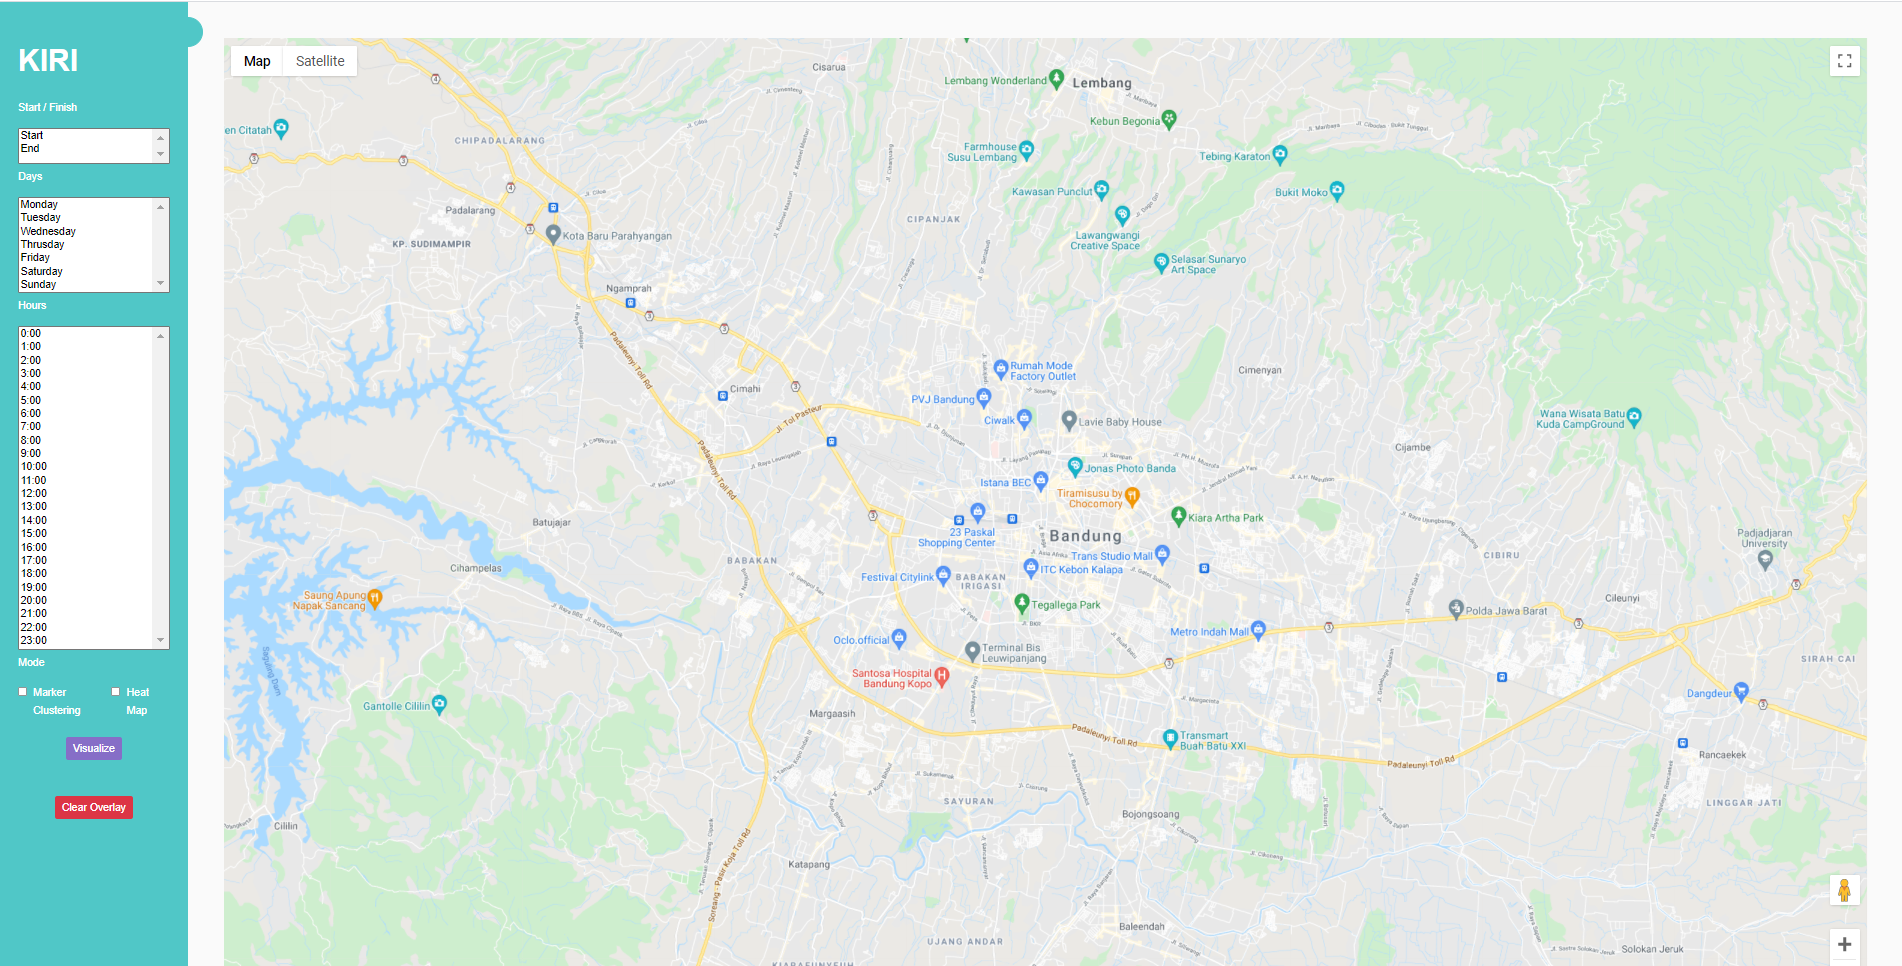
\includegraphics[scale=0.3]{Gambar/Kiri_Ui.PNG}  
	\caption[Tampilan Awal Antarmuka]{Tampilan Awal Antarmuka} 
	\label{fig:interface1} 
\end{figure}

\begin{figure}[H]
	\centering  
	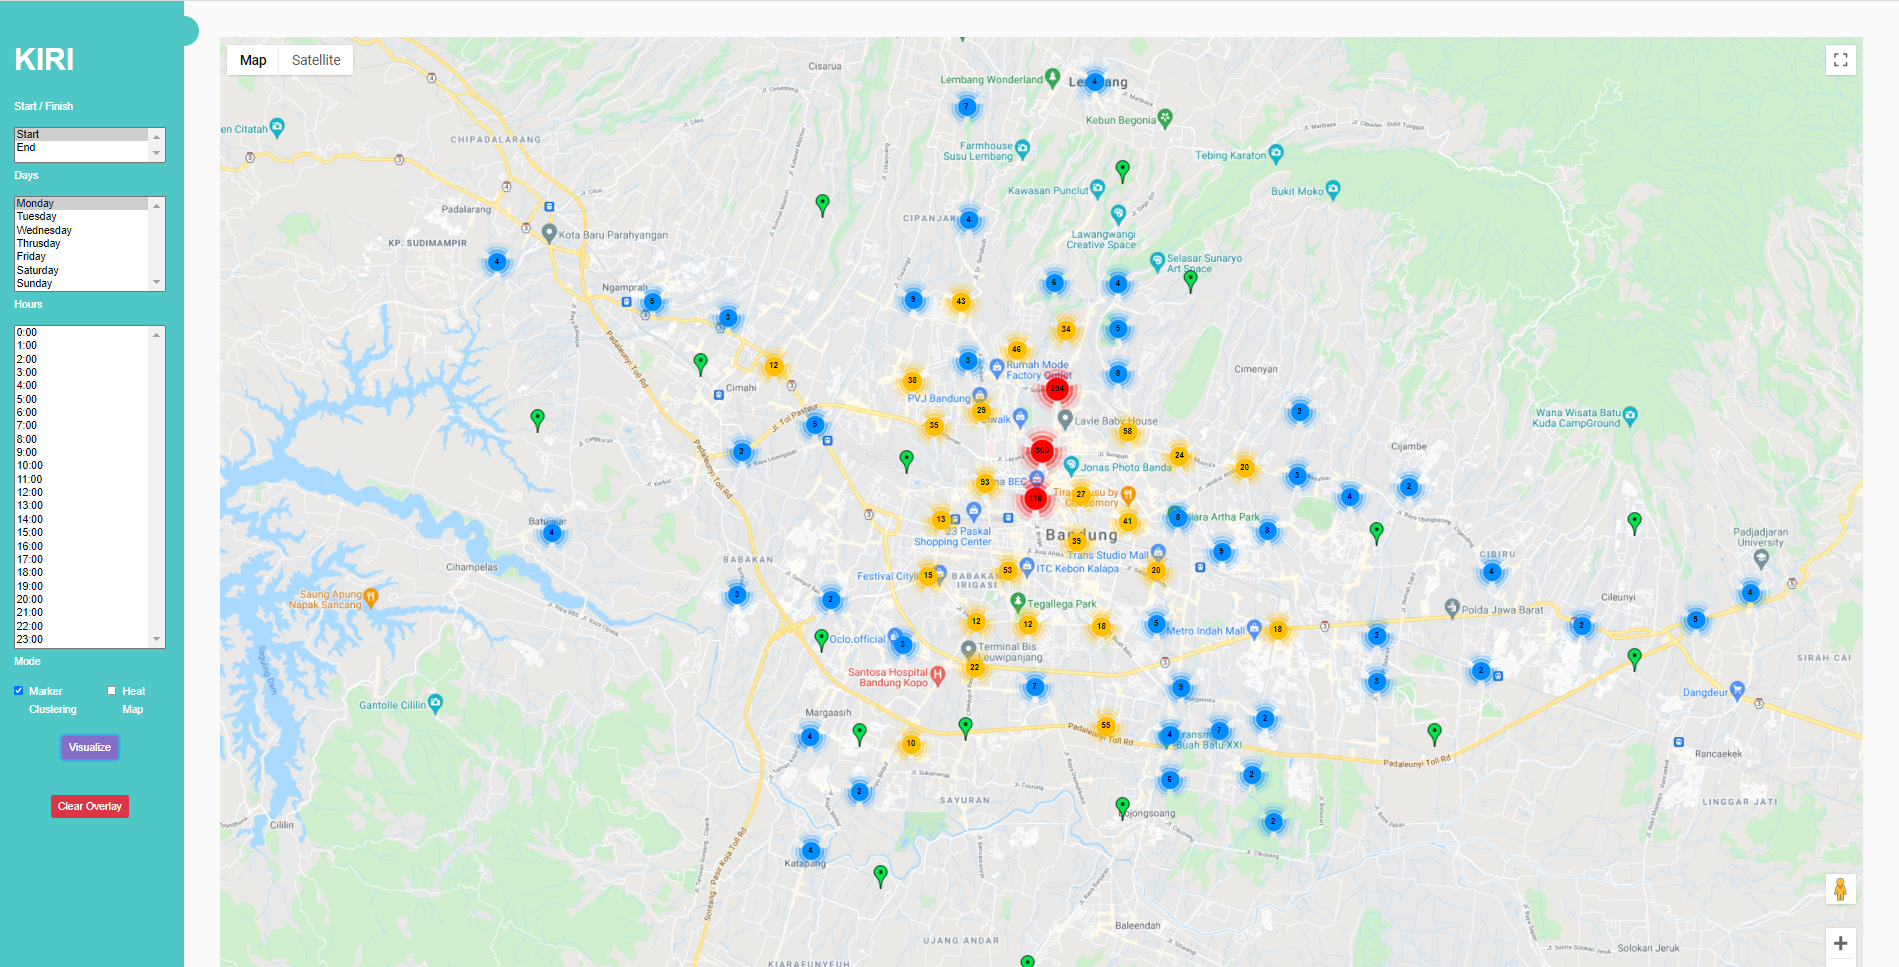
\includegraphics[scale=0.3]{Gambar/Kiri_Ui_Marker.PNG}  
	\caption[Tampilan setelah memilih marker clustering ]{Tampilan setelah memilih marker clustering} 
	\label{fig:interface2} 
\end{figure}

\begin{figure}[H]
	\centering  
	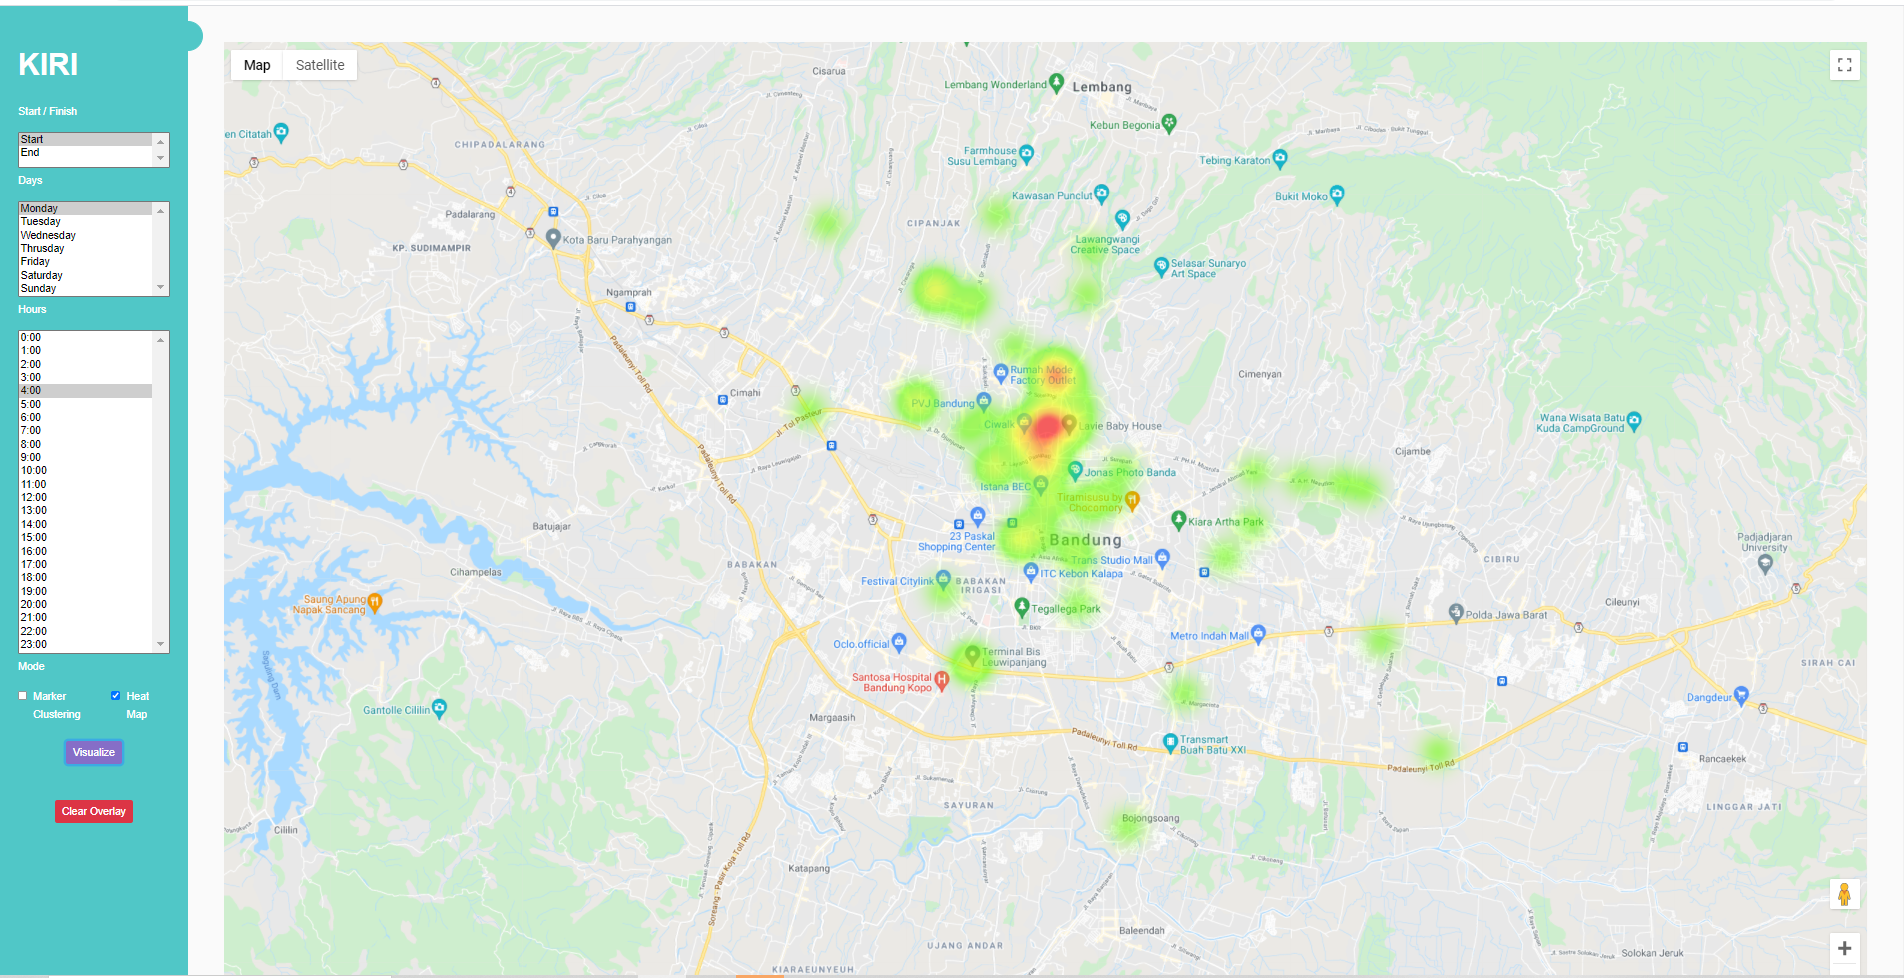
\includegraphics[scale=0.3]{Gambar/Kiri_Ui_Heat_Map.PNG}  
	\caption[Tampilan setelah memilih Heat Map]{Tampilan setelah memilih Heat Map} 
	\label{fig:interface3} 
\end{figure}

\subsection{Implementasi Perangkat Lunak}
Perangkat lunak yang dibuat sesuai dengan perancangan pada Bab \ref{chap:perancangan}. Implementasi aplikasi ini menggunakan bahasa pemrograman \textit{Javascript}. Terdapat tiga bagian utama dalam perangkat lunak yang dibuat.

\begin{itemize}
    \item \textit{Model}\\
    Bagian ini adalah representasi dari data, bagian ini juga dapat disebut sebagai \textit{backend}. Pada bagian ini terdapat kelas \textit{model} untuk data histori KIRI. Pada bagian ini juga terdapat kelas \textit{helper} untuk melakukan operasi pengolahan data.
    \item \textit{Router} \\
    Bagian ini adalah bagian yang menjadi \textit{controller} dalam perangkat lunak. \textit{Router} akan berguna sebagai \textit{media} komunikasi antara \textit{web client} dengan \textit{backend server} 
    \item \textit{View} \\
    Bagian ini adalah bagian tampilan atau yang bisa disebut \textit{web client} karena pada perangkat lunak ini menggunakan\textit{ platfrom website}. Bagian ini bertugas untuk menampilkan hasil visualisasi dan mengolah input dari user.
\end{itemize}

\subsubsection{Model}
Bagian ini adalah representasi dari data, bagian ini juga dapat disebut sebagai \textit{backend}. Pada bagian ini terdapat kelas \textit{model} untuk data histori KIRI. Pada bagian ini juga terdapat kelas \textit{helper} untuk melakukan operasi pengolahan data. Berikut ini adalah gambaran kelas \textit{model} data histori KIRI:

\begin{lstlisting}[label=Kiri_Model, language=JavaScript, caption=Metode Load Data, breaklines]
const fs = require("fs")
const {csvToObject, buildFilter, filterData} = require("./Utils");

class KiriHistory {
    constructor() {
        fs.readFile(__dirname + "/data/KIRIStatistics.csv", "utf8", ((err, data) => {
            if (err === null) {
                let arrCSV = data.split("\n")
                arrCSV.shift();
                this.data = arrCSV.map(csvToObject).filter(item => item !== undefined);
            }
        }))
    }

    //return promise
    getData = (filterParams) => {
        let query = buildFilter(filterParams);
        this.data = filterData(this.data, query);
        return this.data;
    }

}

module.exports = KiriHistory;

\end{lstlisting}

Pada kelas Model ini memiliki tiga \textit{action} utama yaitu:
\begin{enumerate}
    \item {\textbf{Load Data}} \\
Action ini akan dijalankan begitu \textit{object} \textit{model} dibuat. Action ini akan melakukan load dan normalisasi data histori KIRI. Action ini akan menggunakan method \textit{readFile} yang berasal dari \textit{package filesystem}. Berikut ini adalah contoh implementasi dari action ini.


\begin{lstlisting}[label=Kiri_Model, language=JavaScript, caption=Metode Load Data, breaklines]
constructor() {
fs.readFile(__dirname + "/data/KIRIStatistics.csv", "utf8", ((err, data) => {
    if (err === null) {
        let arrCSV = data.split("\n")
        arrCSV.shift();
        this.data = arrCSV.map(csvToObject).filter(item => item !== undefined);
    }
    }))
}
\end{lstlisting}


Method \textit{readFile} akan melakukan action load pada data histori KIRI pada \ref{sec:analisisDataHistoriKiri}. Data yang akan diload bertipe \textit{csv} dan memiliki format data sebagai berikut.
\begin{lstlisting}[label=Kiri_Histori_Data, caption=Histori Data KIRI]
logId,APIKey,Timestamp (UTC),Action,AdditionalData
113909,E5D9904F0A8B4F99,2/1/2014 0:07,PAGELOAD,/5.10.83.30/
113914,A44EB361A179A49E,2/1/2014 0:11,SEARCHPLACE,taman+fot/10
113915,A44EB361A179A49E,2/1/2014 0:11,FINDROUTE,"-6.8972513,107.6385574/-6.91358,107.62718/1"
114256,308201BB30820124,2/1/2014 5:24,SEARCHPLACE,soekarno+hatta+643/10
\end{lstlisting}
Ketika \textit{readFile} dijalankan fungsi ini akan memiliki \textit{callback} yang akan mengembalikan data histori KIRI, data yang telah diload oleh \textit{readFile} akan berbentuk seperti berikut. 
\begin{lstlisting}[label=load_data_1 , caption=Raw Data]
[
 'logId,APIKey,Timestamp (UTC),Action,AdditionalData\r',
  '113909,E5D9904F0A8B4F99,2/1/2014 0:07,PAGELOAD,/5.10.83.30/\r',
  '113910,E5D9904F0A8B4F99,2/1/2014 0:07,PAGELOAD,/5.10.83.49/\r',
  '113911,E5D9904F0A8B4F99,2/1/2014 0:09,PAGELOAD,/5.10.83.30/\r',
]
\end{lstlisting}
Data tersebut akan ditampung ke dalam variabel yang diberi nama \textit{arrCSV}. Baris pertama dari data ini adalah \textit{header} dari csv. Pada proses normalisasi data baris pertama ini tidaklah dibutuhkan oleh karena itu akan dihilangkan baris pertama menggunakan method \textit{shift()}. Sehingga data akan berbentuk sebagai berikut.
\begin{lstlisting}[label=load_data_2 , caption=Raw Data 2]
[
  '113909,E5D9904F0A8B4F99,2/1/2014 0:07,PAGELOAD,/5.10.83.30/\r',
  '113910,E5D9904F0A8B4F99,2/1/2014 0:07,PAGELOAD,/5.10.83.49/\r',
  '113911,E5D9904F0A8B4F99,2/1/2014 0:09,PAGELOAD,/5.10.83.30/\r',
]
\end{lstlisting}
Data tersebut kemudian akan dipetakan ke dalam \textit{map} dengan menggunakan fungsi \textit{mapper} yang diberi nama \textit{csvToObject}. Fungsi ini akan memetakan dan melakukan \textit{formatting} dari setiap \textit{value} dari \ref{load_data_2}.

\begin{lstlisting}[label=helper_1 , caption=CSV Mapper]
const csvToObject = item => {
    let cols = item.split(",")
    let action = cols[3];
    if (action === "FINDROUTE") {
        let startLng = cols[5].split("/")[0]
        let endLat = cols[5].split("/")[1]
        let fullDate = new Date(cols[2])
        return {
            apiKey: cols[0],
            timestamp: fullDate,
            action,
            startCor: {lat: parseFloat(cols[4].substr(1)), lng: parseFloat(startLng)},
            endCor: {lat: parseFloat(endLat), lng: parseFloat(cols[6].split("/")[0])},
            day: fullDate.getDay(),
            hour: fullDate.getHours()
        }
    }
}
\end{lstlisting}

Fungsi ini akan akan memanfaatkan \textit{method split} untuk membagi raw data \ref{load_data_2} menjadi array yang berbentuk seperti berikut.

\begin{lstlisting}[label=data_parser_1 , caption=Data Split Result]
[
  '115566',
  'A44EB361A179A49E',
  '2/2/2014 9:07',
  'FINDROUTE',
  '"-0.7819376',
  '100.2871169/-6.90359',
  '107.60040/1"\r'
]

\end{lstlisting}
Berdasarkan data \ref{data_parser_1} kita dapat mengekstrak  \textit{action type} \ref{sec:analisisDataHistoriKiri} pada posisi ketiga dari array tersebut. Dalam aplikasi ini hanya akan digunakan data yang memiliki \textit{action} \textit{FINDROUTE} hal ini dikarenakan hanya pada \textit{action} ini data mengandung \textit{value} dari posisi \textit{start} dan \textit{finish}. Setelah function \textit{csvToObject} ini dijalankan maka akan mengembalikan kumpulan \textit{object} data yang berbentuk sebagai berikut.

\begin{lstlisting}[label=data_parser_result , caption=Result Data]
[
    {
      apiKey: '113915',
      timestamp: 2014-01-31T17:11:00.000Z,
      action: 'FINDROUTE',
      startCor: { lat: -6.8972513, lng: 107.6385574 },
      endCor: { lat: -6.91358, lng: 107.62718 },
      day: 6,
      hour: 0
    }
]
\end{lstlisting}

\item{\textbf{Get Data}} \\
Fungsi ini akan dijalankan setiap ada request dari \textit{web client}. \textit{Action} ini akan mengembalikan data histori KIRI sesuai dengan filter parameter yang diberikan. Berikut ini adalah contoh implementasi dari \textit{action} ini.
\begin{lstlisting}[label=get_data , caption=Function Get Data]
    getData = (filterParams) => {
        let query = buildFilter(filterParams);
        this.data = filterData(this.data, query);
        return this.data;
    }
\end{lstlisting}
Pada fungsi ini akan menerima parameter \textit{filterParams} yang berasal dari \textit{web client}. Fungsi ini akan menjalankan dua perintah yaitu \textit{buildFilter} dan  \textit{filterData} dan akan mengembalikan data histori yang sesuai dengan \textit{filterParams} yang diberikan. Fungsi \textit{buildFilter} akan mengubah \textit{filterParams} yang berbentuk seperti berikut.
\begin{lstlisting}[label=filter_params , caption=Filter Parameter]
{
    day: [ 0 ], 
    hour: [ 8, 9, 10, 11 ] 
}
\end{lstlisting}
Menjadi \textit{query params}. Hal ini dilakukan karena fungsi \textit{filter} yang dirancang pada perangkat lunak ini akan memanfaatkan \textit{function} filter dari javascript.

\item{Filter Data} \\
Berikut ini adalah hasil implementasi dari \textit{function filter}:
\begin{lstlisting}[label=filter_method , caption=Fungsi Filter]
 const filterData = (data, query) => {
    const keysWithMinMax = [];
    const filteredData = data.filter((item) => {
        for (let key in query) {
            if (item[key] === undefined) {
                return false;
            } else if (keysWithMinMax.includes(key)) {
                if (query[key]['min'] !== null && item[key] < query[key]['min']) {
                    return false;
                }
                if (query[key]['max'] !== null && item[key] > query[key]['max']) {
                    return false;
                }
            } else if (!query[key].includes(item[key])) {
                return false;
            }
        }
        return true;
    });
    return filteredData;
};
\end{lstlisting}

Fungsi ini akan memanfaatkan \textit{method filter} dan \textit{includes javascript}. Fungsi ini akan menghasilkan data yang telah disaring sesuai dengan \textit{query params} yang diberikan.
 \end{enumerate}

\subsubsection{Router}
Bagian ini merupakan bagian yang bertugas sebagai \textit{controller} antara \textit{backend logic} dan \textit{web client}. Implementasi router dapat dilihat sebagai berikut.

\lstinputlisting[label=Router , caption=Router Implementation]{./Lampiran/app/route.js} 

Bagian ini memiliki dua fungsi utama yaitu melakukan render untuk \textit{web client} dan mengatur \textit{response} dan \textit{request} antara \textit{web client} dan \textit{backend logic}.

\begin{enumerate}
    \item \textbf{Render HTML} \\
Perangkat lunak ini menggunakan \textit{node.js} sebagai \textit{runtime manager}. Perangkat lunak ini memanfaatkan \textit{method sendFile} milik \textit{node.js} untuk dapat melakukan \textit{rendering} pada \textit{route} yang diinginkan. Implementasi pada bagian ini dapat dilihat sebagai berikut.

\begin{lstlisting}[label=render_html , caption=Render HTML]
app.get("/", (req, res) => {
    res.sendFile(path.join(`${viewPath}/index.html`));
})
\end{lstlisting}
Pada potongan kode diatas menunjukan bahwa \textit{index.html} akan dirender pada \textit{route '/'}.

\item \textbf{\textit{Controller} antara \textit{Web client} dan \textit{Backend Logic}} \\
Implementasi pada bagian ini dapat dilihat sebagai berikut.
\begin{lstlisting}[label=render_html , caption=Get Filtered Data]
app.post('/searchRoute', (req, res) => {
    let filterParams = req.body;
    let data = modelKiri.getData(filterParams);
    res.status(200).json({
        'status': 'OK',
        'messages': 'Data',
        'data': data,
    })

})
\end{lstlisting}

Pada bagian ini perangkat lunak akan membuat \textit{endpoint} yang akan menerima parameter berupa \textit{filter parameter} dan akan mengembalikan hasil data histori yang telah difilter.
\end{enumerate}

\subsubsection{View}
Bagian ini adalah bagian disebut \textit{web client} pada \ref{sec:webclientCapability}. Pada bagian ini terdapat fungsi untuk menerima \textit{input user} dan menampilkan hasil visualisasi menggunakan \textit{Google Maps Javascript API}. Pada bagian ini format \textit{user interface} akan ditulis dalam  format \textit{Hypertext Markup Language (html)} hal ini dapat dilihat pada file \textit{index.html}.
Selain untuk tampilan bagian ini juga berfungsi untuk menerima input user dan mengubahnya menjadi \textit{filter params}, hal ini dapat dilihat pada file \textit{maps.js}. Bentuk implementasi dari bagian ini dapat dilihat sebagai berikut.

\lstinputlisting[label=Map , caption=Map Implementation]{./Lampiran/app/maps.js} 

Bagian ini memiliki tiga tugas utama yaitu:
\begin{enumerate}
    \item \textbf{Menerima \textit{input user} dan mengubah \textit{input user} menjadi \textit{filter params}} \\
Implementasi bagian ini dapat dilihat menjadi:
\begin{lstlisting}[label=input_user , caption=Input User]
createFilterObj = () => {
    let days = Array.from(document.getElementById("day").selectedOptions).map(option => parseInt(option.value))
    let hours = Array.from(document.getElementById("hour").selectedOptions).map(option => parseInt(option.value));
    let filter = {day: days, hour: hours}
    return filter
}

\end{lstlisting}

Ketika fungsi ini dijalankan maka akan mengambil \textit{value} dari elemen dengan id \textit{day} dan \textit{hour}. Setelah itu data tersebut akan dibuat ke dalam bentuk \textit{map} yang disebut sebagai \textit{filter parameter}. Pada bagian ini juga terdapat fungsi \textit{docReady} yang bertugas untuk  berkomunikasi dengan \textit{node.js} atau \textit{Google Maps Javascript API}. Hasil implementasi fungsi tersebut adalah sebagai berikut:
\begin{lstlisting}[label=docReady , caption=docReady Method]
function docReady(fn) {
    if (document.readyState === "complete" || document.readyState === "interactive") {
        setTimeout(fn, 1);
    } else {
        document.addEventListener("DOMContentLoaded", fn);
    }
}

\end{lstlisting}
Pada fungsi ini memiliki parameter sebuah fungsi dimana fungsi ini akan dijalankan setiap \textit{tick}. Hal ini dilakukan agar koneksi antar \textit{backend} bisa tetap terus dilakukan. Berikut ini implementasi fungsi \textit{docReady} pada perangkat lunak ini.

\begin{lstlisting}[label=docReady_1 , caption=docReady Method]
docReady(function () {
    let map = initMap()
    let markerCluster = null;
    let markers;
    let heatMap;
    document.getElementById("send-btn").onclick = function (e) {
        e.preventDefault();
        let filterParams = createFilterObj()
        let isMarkerCluster = document.getElementById("marker-cluster").checked
        let isHeatMap = document.getElementById("heat-map").checked
        let statusSelected = Array.from(document.getElementById("start-finish").selectedOptions).map(option => option.value)
        let statusStartChecked = statusSelected.includes("start");
        let statusEndChecked = statusSelected.includes("end")
        sendRequest("http://localhost:3000/searchRoute", filterParams).then(res => {
            if (isMarkerCluster) {
                map.setMapTypeId(google.maps.MapTypeId.ROADMAP);
                let data = res.data.data;
                if (!Array.isArray(markers)) {
                    markers = setMarkers(data, statusStartChecked, statusEndChecked)
                    markerCluster = new MarkerClusterer(map, markers, {
                        imagePath:
                            "https://developers.google.com/maps/documentation/javascript/examples/markerclusterer/m",
                    });
                }
            }

            if (isHeatMap) {
                map.setMapTypeId(google.maps.MapTypeId.ROADMAP);
                if (!heatMap || heatMap.getMap() === null) {
                    heatMap = setHeatMap(res.data.data, map, statusStartChecked, statusEndChecked)
                }
            }
        });
    }

    document.getElementById('clear-btn').onclick = function (e) {
        e.preventDefault();
        if (markerCluster) {
            markerCluster.removeMarkers(markers);
            markers = deleteMarkes(markers)
        }
        if (heatMap) {
            heatMap.setMap(null)
        }
    }
});

\end{lstlisting}

\item \textbf{Mengirim dan menerima data dari router} \\
Implementasi untuk bagian ini dapat dilihat pada \textit{method} docReady.

\begin{lstlisting}[label=communication , caption=communication method]
    document.getElementById("send-btn").onclick = function (e) {
        e.preventDefault();
        let filterParams = createFilterObj()
        let isMarkerCluster = document.getElementById("marker-cluster").checked
        let isHeatMap = document.getElementById("heat-map").checked
        let statusSelected = Array.from(document.getElementById("start-finish").selectedOptions).map(option => option.value)
        let statusStartChecked = statusSelected.includes("start");
        let statusEndChecked = statusSelected.includes("end")
        sendRequest("http://localhost:3000/searchRoute", filterParams).then(res => {
            if (isMarkerCluster) {
                map.setMapTypeId(google.maps.MapTypeId.ROADMAP);
                let data = res.data.data;
                if (!Array.isArray(markers)) {
                    markers = setMarkers(data, statusStartChecked, statusEndChecked)
                    markerCluster = new MarkerClusterer(map, markers, {
                        imagePath:
                            "https://developers.google.com/maps/documentation/javascript/examples/markerclusterer/m",
                    });
                }
            }

            if (isHeatMap) {
                map.setMapTypeId(google.maps.MapTypeId.ROADMAP);
                if (!heatMap || heatMap.getMap() === null) {
                    heatMap = setHeatMap(res.data.data, map, statusStartChecked, statusEndChecked)
                }
            }
        });
    }
\end{lstlisting}

Pada potongan kode di atas dapat dilihat jika tombol send-btn ditekan, maka akan memanggil method \textit{sendRequest}. Method ini bertujuan untuk berkomunikasi dengan \textit{backend} untuk mendapatkan data yang histori yang telah disaring berdasarkan input dari user. Fungsi ini juga bertujuan untuk mendapatkan hasil visualisasi dari data yang telah disaring dengan menggunakan \textit{Google Maps Javascript API}.

\item\textbf{Berkomunikasi dengan \textit{Google Maps Javascript API}} \\
Perangkat lunak ini menggunakan \textit{Google Maps Javascript API} sebagai salah satu \textit{third party library} untuk melakukan visualisasi data. Terdapat dua buah opsi yang disediakan oleh perangkat lunak ini dalam melakukan visualisasi data yaitu \textit{Heat Map} dan \textit{Marker Clustering}. Untuk dapat menggunakan opsi tersebut \textit{web client} perlu membuat input parameter yang sesuai dengan kebutuhan \textit{Google Maps Javascript API} \ref{sec:googlemaps}. Implementasi dari bagian ini dapat dilihat sebagai berikut.

\begin{lstlisting}[label=map_input , caption=Map Input]
function setMarkers(data, isStart, isEnd) {
    let locations = [];
    if (isStart) {
        data.forEach(item => {
            let startMark = {
                name: "start",
                pos: item.startCor,
                icon: "http://maps.google.com/mapfiles/ms/icons/green-dot.png"
            }
            locations.push(startMark)
        })
    }

    if (isEnd) {
        data.forEach(item => {
            let endMark = {name: "end", pos: item.endCor, icon: "http://maps.google.com/mapfiles/ms/icons/red-dot.png"}
            locations.push(endMark)
        })
    }

    // console.log("filtered markers size" , data.length)
    let markers = locations.map((item) => {
        return new google.maps.Marker({
            position: {lat: parseFloat(item.pos.lat), lng: parseFloat(item.pos.lng)},
            icon: item.icon
        });
    });
    return markers;
}


function setHeatMap(arrData, map, isStart, isEnd) {
    let heatmapData = [];
    if (isStart) {
        arrData.forEach(item => {

            let startCoor = {location: new google.maps.LatLng(item.startCor.lat, item.startCor.lng)}
            heatmapData.push(startCoor)

        })
    }
    if (isEnd) {
        arrData.forEach(item => {
            // {location: new google.maps.LatLng(37.782, -122.447), weight: 0.5},
            let endLocationObj = {location: new google.maps.LatLng(item.endCor.lat, item.endCor.lng)}
            heatmapData.push(endLocationObj)
        })
    }

    let heatmap = new google.maps.visualization.HeatmapLayer({
        data: heatmapData,
        radius: 50
    });
    heatmap.setMap(map);

    return heatmap;
}

\end{lstlisting}
\end{enumerate}

\section{Pengujian}
\label{sec:pengujian}
Pengujian dilakukan dengan menggunakan dua metode yaitu pengujian fungsional dan pengujian eksperimental. Pengujian fungsional bertujuan untuk menguji fitur-fitur yang telah disediakan. Pengujian Eksperimental bertujuan untuk mencari pola-pola tertentu pada data histori KIRI.

\subsection{Pengujian Fungsional}
Pengujian fungsional dilakukan dengan menjalankan fitur-fitur yang ada. Berikut adalah fitur-fitur yang ada pada perangkat lunak.
\begin{enumerate}
	\item Filter Data Histori KIRI\\
	Fitur ini bertujuan untuk melakukan proses filterisasi pada data histori KIRI sesuai dengan input yang diberikan pengguna. Pengguna dapat memasukan tiga jenis empat jenis input sesuai dengan yang telah disediakan pada tampilan \ref{fig:filterState}, pengguna dapat melakukan filter berdasarkan atribute \textit{day} dapat dilihat pada kotak bewarna merah, \textit{hour} dapat dilihat pada kotak bewarna \textit{orange}, dan \textit{start/finsih} dapat dilihat pada kotak bewarna hitam.
	
	\begin{figure}[H]
	\centering  
	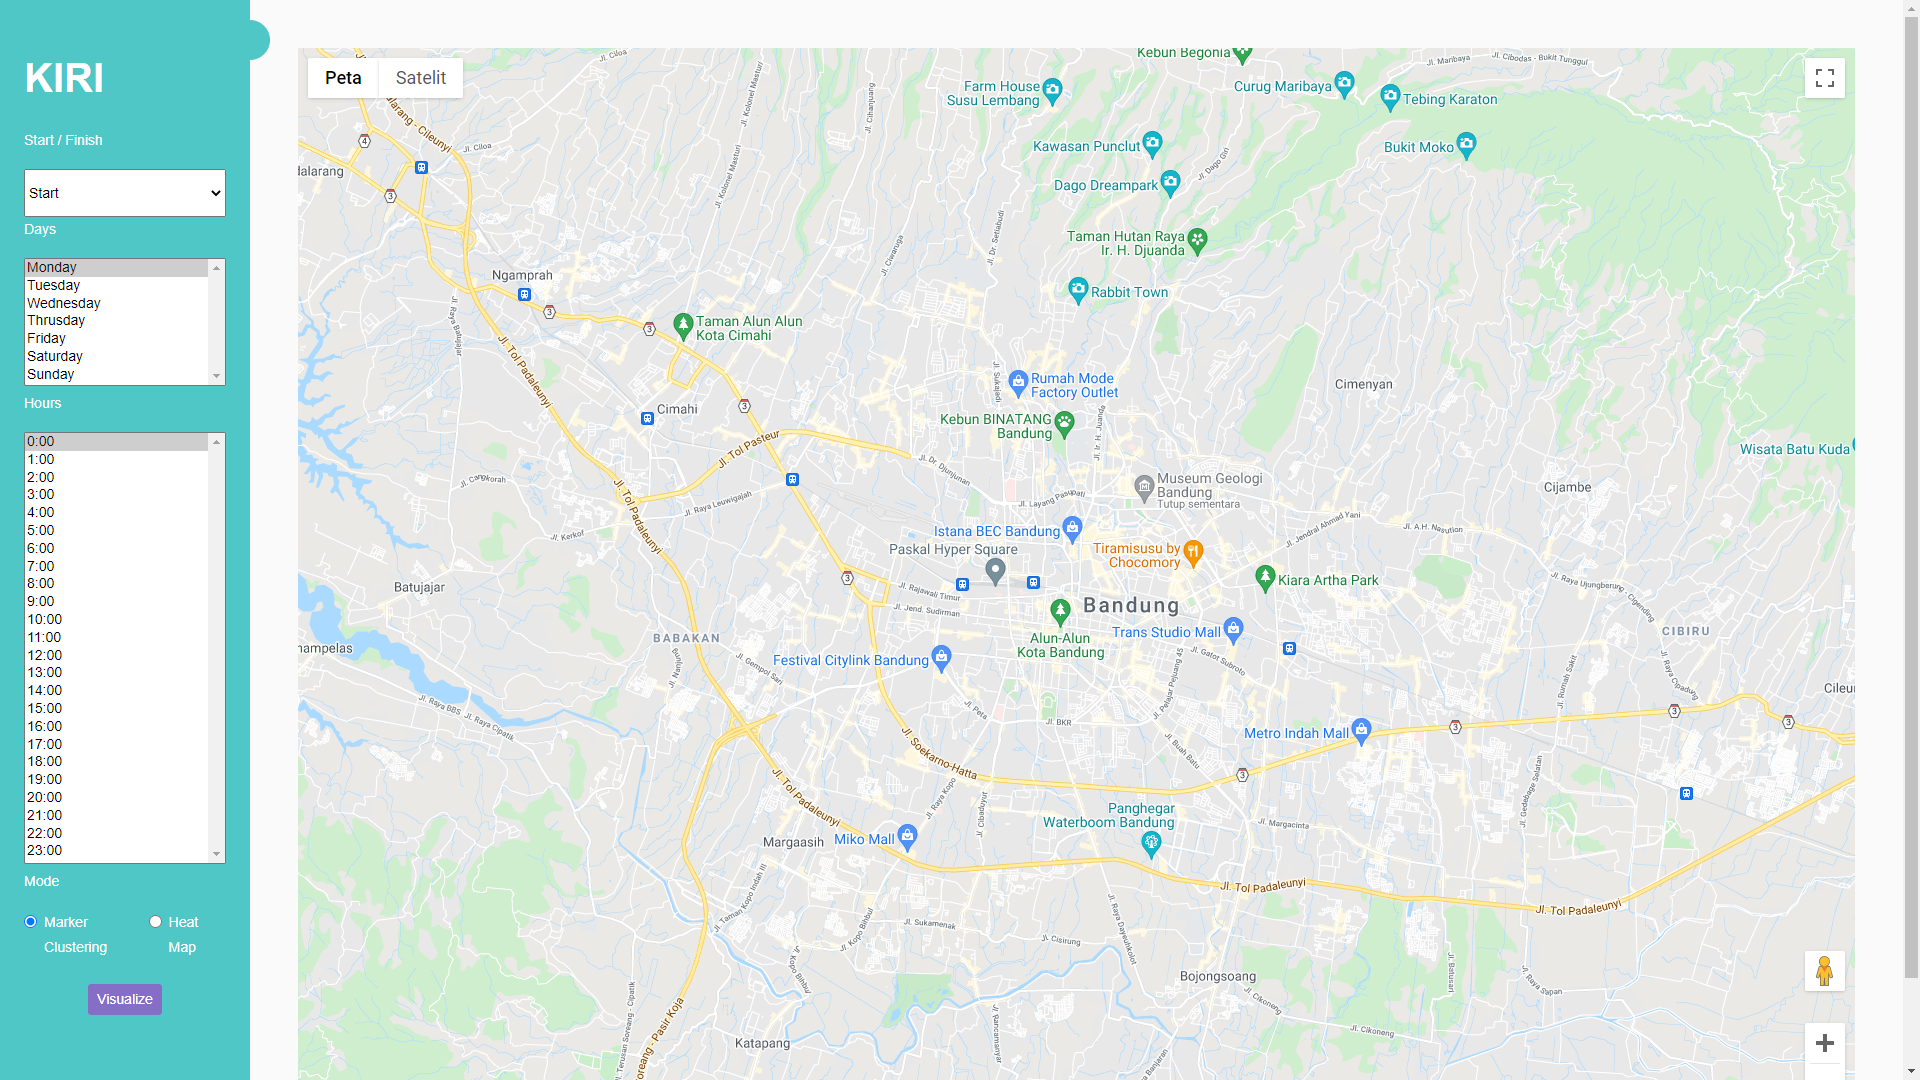
\includegraphics[scale=0.3]{Gambar/KIRI-UI.png}  
	\caption[Tampilan Filter Data Histori KIRI]{Tampilan Filter Data Histori KIRI} 
	\label{fig:filterState}
	\end{figure}
	
	\item Menampilkan visualisasi data dalam bentuk \textit{marker}\\
	Fitur ini bertujuan untuk memvisualisasikan data dalam bentuk \textit{marker}. Jika pengguna memilih \textit{option} \textit{marker clustering} dan menekan tombol \textit{visualize}, maka program akan menampilkan data dalam bentuk \textit{marker} pada \textit{object} \textit{map} seperti Gambar \ref{fig:markerState}.
	
	\begin{figure}[H]
	\centering  
	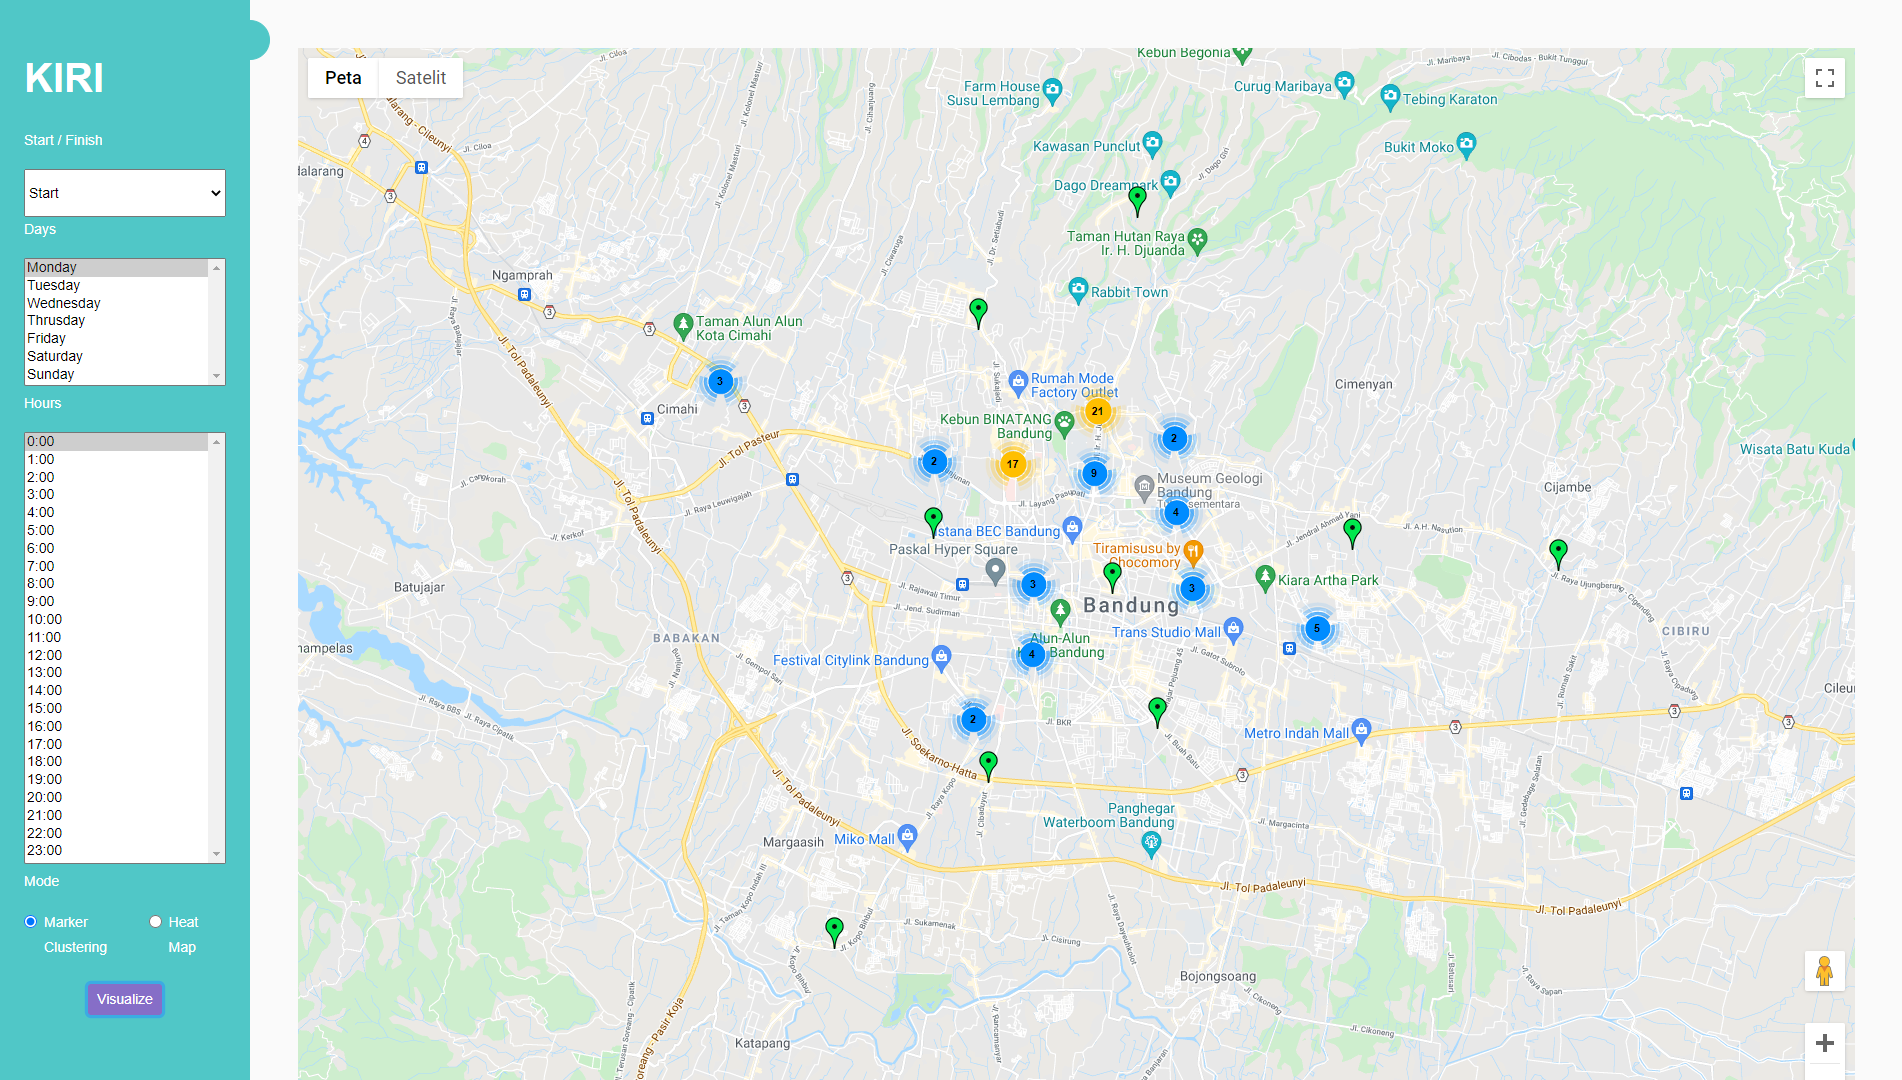
\includegraphics[scale=0.3]{Gambar/Kiri-Marker.PNG}  
	\caption[Tampilan Marker Data Histori KIRI]{Tampilan Marker Data Histori KIRI} 
	\label{fig:markerState}
	\end{figure}
	
	\item  Menampilkan visualisasi data dalam bentuk \textit{heat map}\\
	Fitur ini bertujuan untuk memvisualisasikan data dalam bentuk \textit{heat map}. Jika pengguna memilih \textit{option} \textit{heat map} dan menekan tombol \textit{visualize}, maka program akan menampilkan data dalam bentuk \textit{heat map} pada \textit{object} \textit{map} seperti Gambar \ref{fig:heatmapState}.
	
	\begin{figure}[H]
	\centering  
	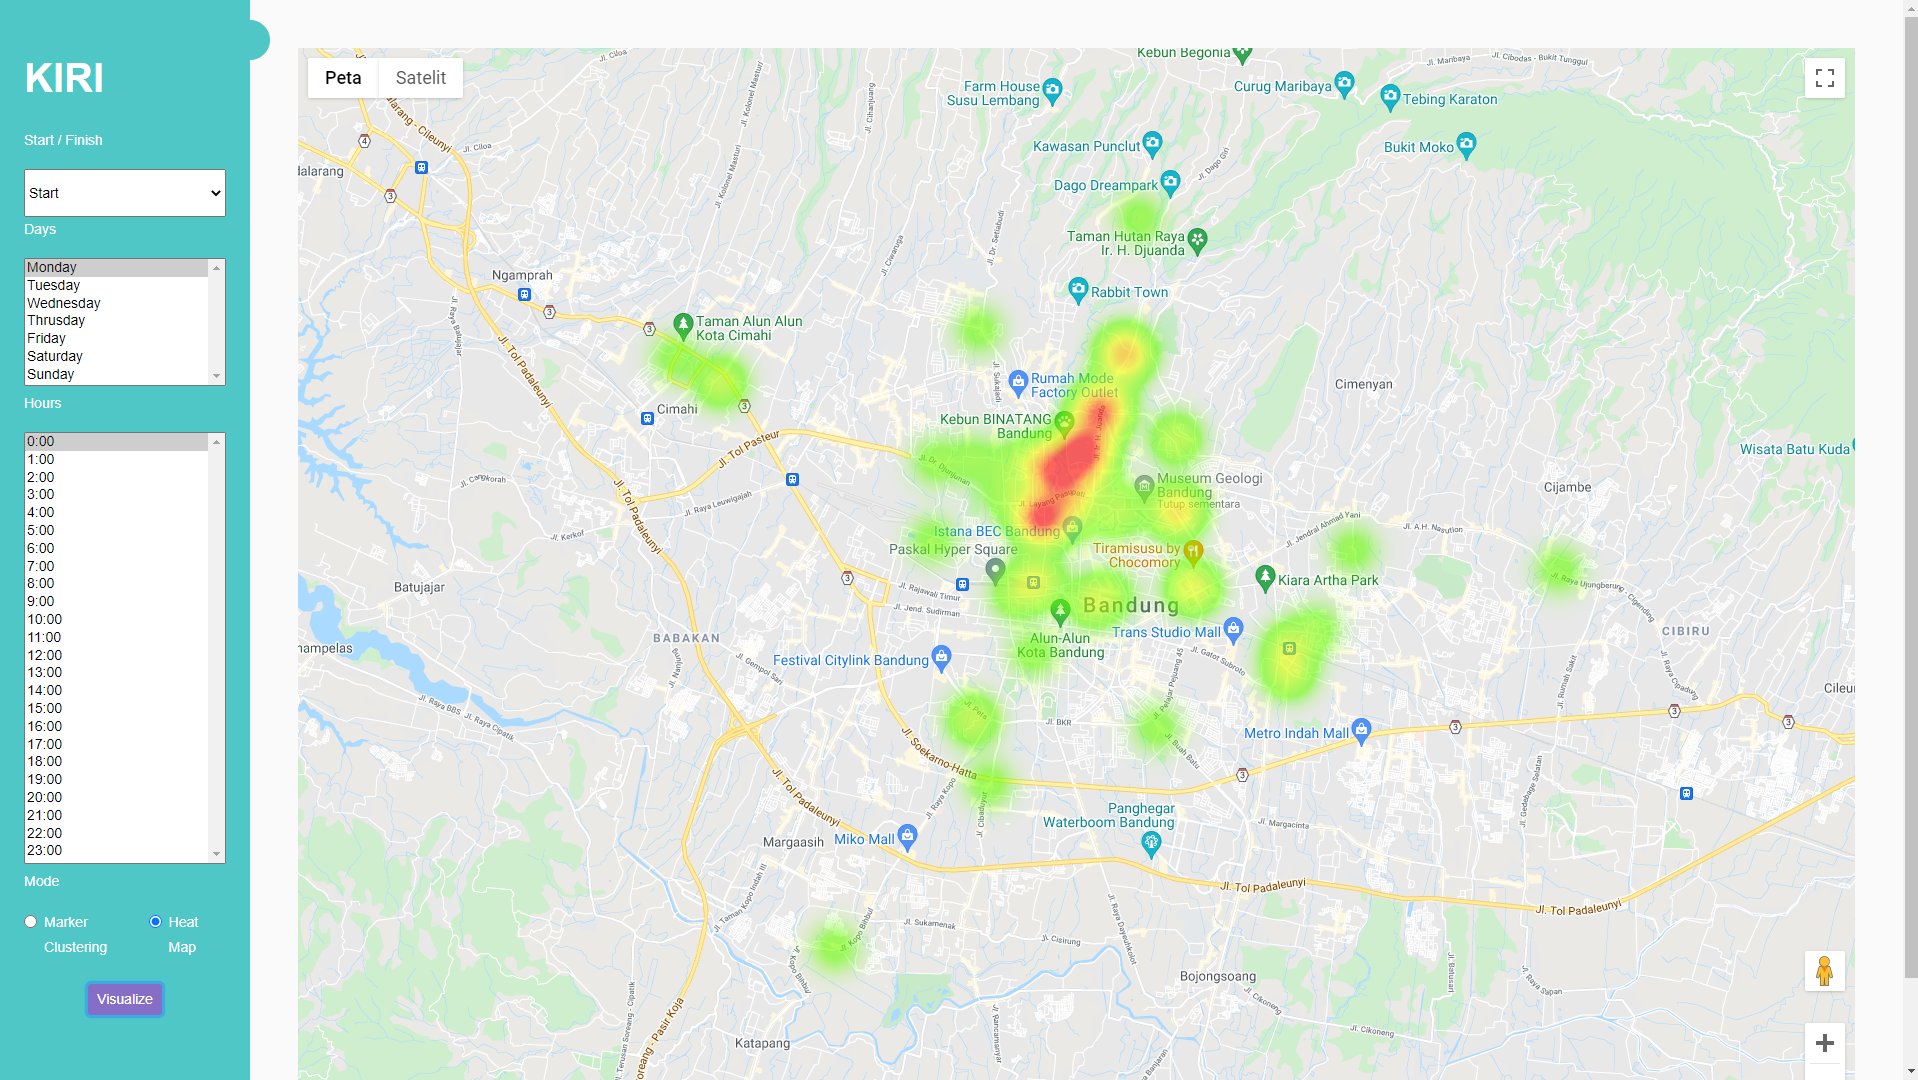
\includegraphics[scale=0.3]{Gambar/Kiri-heat-map.PNG}  
	\caption[Tampilan Heat Map  Histori KIRI]{Tampilan Heat Map  Data Histori KIRI} 
	\label{fig:heatmapState}
	\end{figure}
	
	
\end{enumerate}

Pengujian fungsional pada perangkat lunak ini dilakukan dengan menggunakan\textit{ automated test} dengan bantuan \textit{third party app} \textit{cypress.io}. Pengujian dibagi dalam tiga tahap, yaitu:

\begin{enumerate}
    \item Pengujian tampilan\\
    Pengujian ini bertujuan untuk memastikan tampilan telah tersedia / berhasil ditampilkan pada \textit{web client}. Pengujian dilakukan dengan membuat \textit{test case}:\\
    \begin{lstlisting}[label=ui_test_case , caption=UI Test Case]
    describe('KIRI history html dom end to end testing', () => {
    it('Check website succesfully  loaded ', () => {
        cy.visit(WEB_DOMAIN_NAME)
        cy.get('h1').should('have.text', "KIRI");
    })
    it('Check  start/finish html already exist or already loaded', () => {
        cy.get('#start-finish').select(COMPLETION_STATUS[0]).should('have.value', 'start');
        cy.get('#start-finish').select(COMPLETION_STATUS[1]).should('have.value', 'end');
    })
    it('Check  days  html already exist or already loaded', () => {
        let expectedValue = ['0', "1", "2", "3", "4", "5", "6"];
        cy.get('#day')
            .select(DAYS)
            .invoke('val')
            .should('deep.equal', expectedValue)
    })
    it('Check  time html dom already exist or already loaded', () => {
        let expectedValue = ['0', "1", "2", "3", "4", "5", "6", "7", "8", "9", "10", "11", "12", "13", "14", "15", "16", "17", "18", "19", "20", "21", "22", "23"];
        cy.get('#hour')
            .select(HOURS)
            .invoke('val')
            .should('deep.equal', expectedValue)
    })
    it('Check  visualization mode  html dom already exist or already loaded', () => {
        cy.get('#marker-cluster').check();
        cy.get('#heat-map').click().check();
    })
})

    \end{lstlisting}
    
    \item Pengujian fungsional dengan mengunakan metode \textit{visual regression} \\
    Pengujian ini bertujuan untuk menguji fungsi \textit{heat map} dan \textit{marker clustering} metode yang digunakan adalah membandingkan gambar \textit{map} sebelum dan sesudah pemanggilan fungsi tersebut. \textit{Syntax test case} yang dibuat akan berbentuk seperti berikut.\\
    \begin{lstlisting}[label=functional_test_case_visual , caption=Funcional Test Case Visual Regression]
COMPLETION_STATUS.forEach(status => {
    DAYS.forEach(day => {
        HOURS_TEST.forEach(hour => {
            describe('Functional Testing  check with visual regression', () => {
                it(`Test for marker cluster functional  in status ${status},day ${day},and time ${hour}`, () => {
                    cy.get('#marker-cluster').click();
                    cy.get('#start-finish').select(status).get("#day").select(day);
                    cy.get("#hour").select(hour).get("#send-btn").click().get("#map").notMatchImageSnapshot();

                    cy.get('#start-finish').select(status).get("#day").select(day);
                    cy.get("#hour").select(hour).get("#send-btn").click().get("#map").wait(2000).notMatchImageSnapshot();

                })
            })
        })
    })
})
    \end{lstlisting}
    Pengujian ini akan memiliki hasil seperti pada Gambar \ref{fig:visualRegressionState}.
    \begin{figure}[H]
	\centering  
	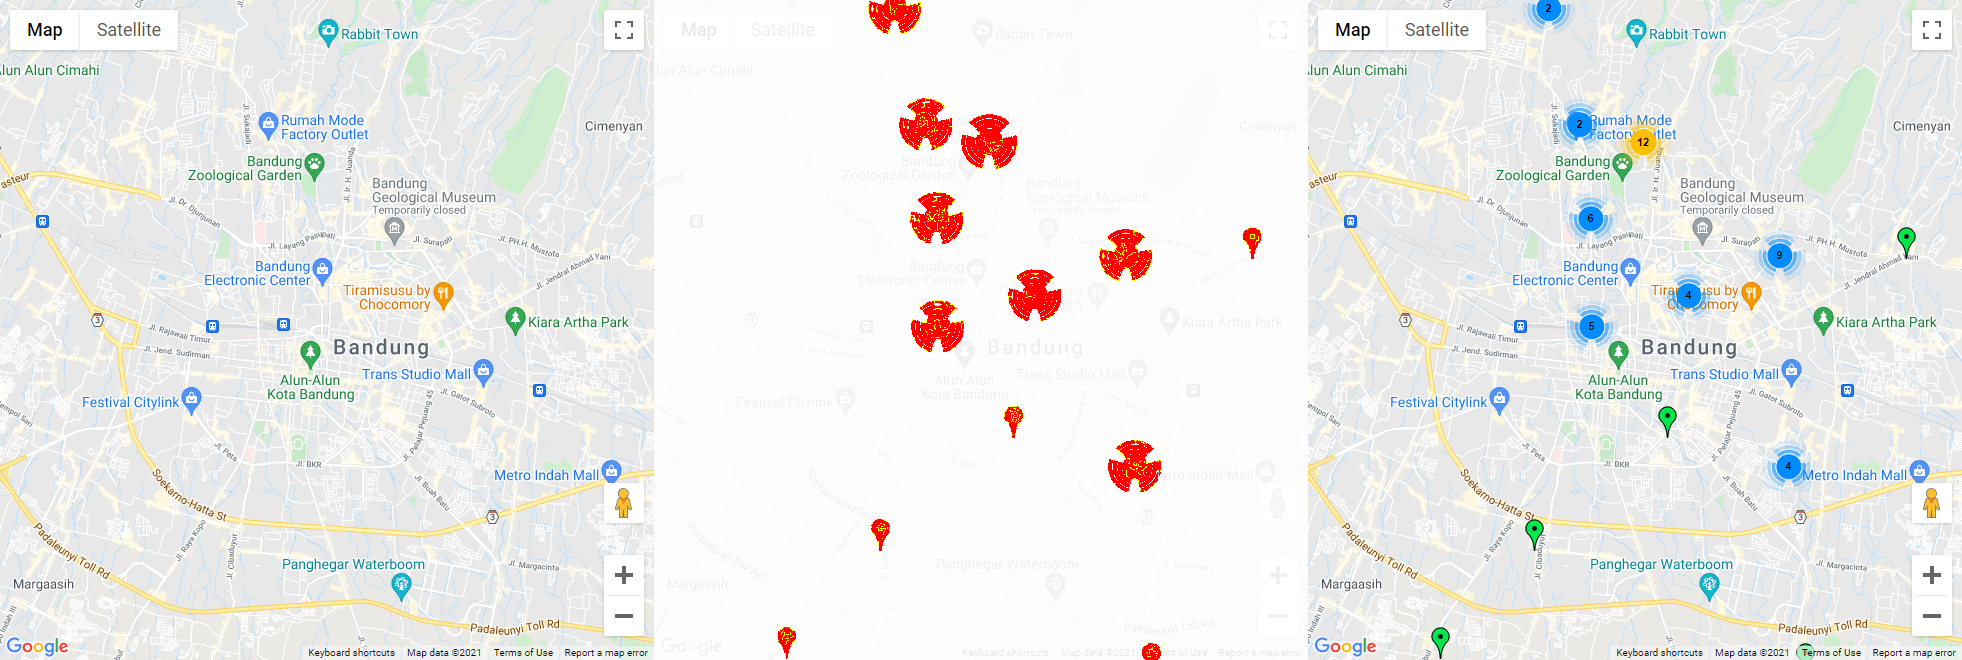
\includegraphics[scale=0.2]{Gambar/Visual_Regression_Sample_Method.png}  
	\caption[Visual regression sample result]{Visual regression sample result} 
	\label{fig:visualRegressionState}
	\end{figure}
	
	
	\item Pengujian fungsional dengan mengunakan metode \textit{http response status} \\
    Pengujian ini bertujuan untuk menguji fungsi \textit{heat map} dan \textit{marker clustering} metode yang digunakan adalah melihat \textit{response} status yang dikeluarkan oleh \textit{node server}. \textit{Syntax test case} yang dibuat akan berbentuk seperti berikut.\\
    \begin{lstlisting}[label=functional_test_case , caption=Funcional Test Case ]
COMPLETION_STATUS.forEach(status => {
    DAYS.forEach(day => {
        HOURS_TEST.forEach(hour => {
            describe("Functional Testing  check with http request status", () => {
                it(`Test for marker cluster in status ${status},day ${day},and time ${hour}`, () => {
                    cy.get('#marker-cluster').click();
                    cy.get('#start-finish').select(status).get("#day").select(day);
                    cy.get("#hour").select(hour).get("#send-btn").click().request('POST', '/searchRoute').then(res =>
                        expect(res.status).to.eq(200)
                    );
                })
            });
        })
    })
})
    \end{lstlisting}
    
\end{enumerate}

Total pengujian yang berjumlah 47 \textit{test case} yang sudah dilengkapi dengan bukti \textit{screenshoot} dan \textit{video} yang dapat diakses pada tautan \href{https://dashboard.cypress.io/projects/cgtb3m/runs/1/overview}{dashboard}.

\subsection{Pengujian Eksperimental}
\label{subsec: pengujian}
Tujuan dari pengujian ini adalah mencari pola-pola tertentu pada data histori KIRI dengan menggunakan metode observasi. Pengujian akan dilakukan untuk menjawab beberapa pertanyaan yaitu:
\begin{enumerate}
    \item Bagaimana pengguaan perangkat lunak KIRI pada saat jam kerja?
    \item Bagaimana pengguaan KIRI pada saat non jam kerja ?
    \item  Daerah manakah  paling sering dijadikan titik awal pencarian rute ?
    \item  Daerah manakah  paling sering dijadikan tujuan akhir pencarian rute ?
    \item Daerah manakah  paling sering dijadikan titik awal pencarian rute pada saat \textit{weekend} ?
    \item Daerah manakah  paling sering dijadikan titik tujuan pencarian rute pada saat \textit{weekend} ?
\end{enumerate}

Untuk membantu menjawab beberapa pertanyaan diatas akan ditambahkan sebuah parameter untuk mengetahui berapa jumlah data yang didapat saat pengguna melakukan visualisasi pada Gambar \ref{fig:testingState}.
   
    \begin{figure}[H]
	\centering  
	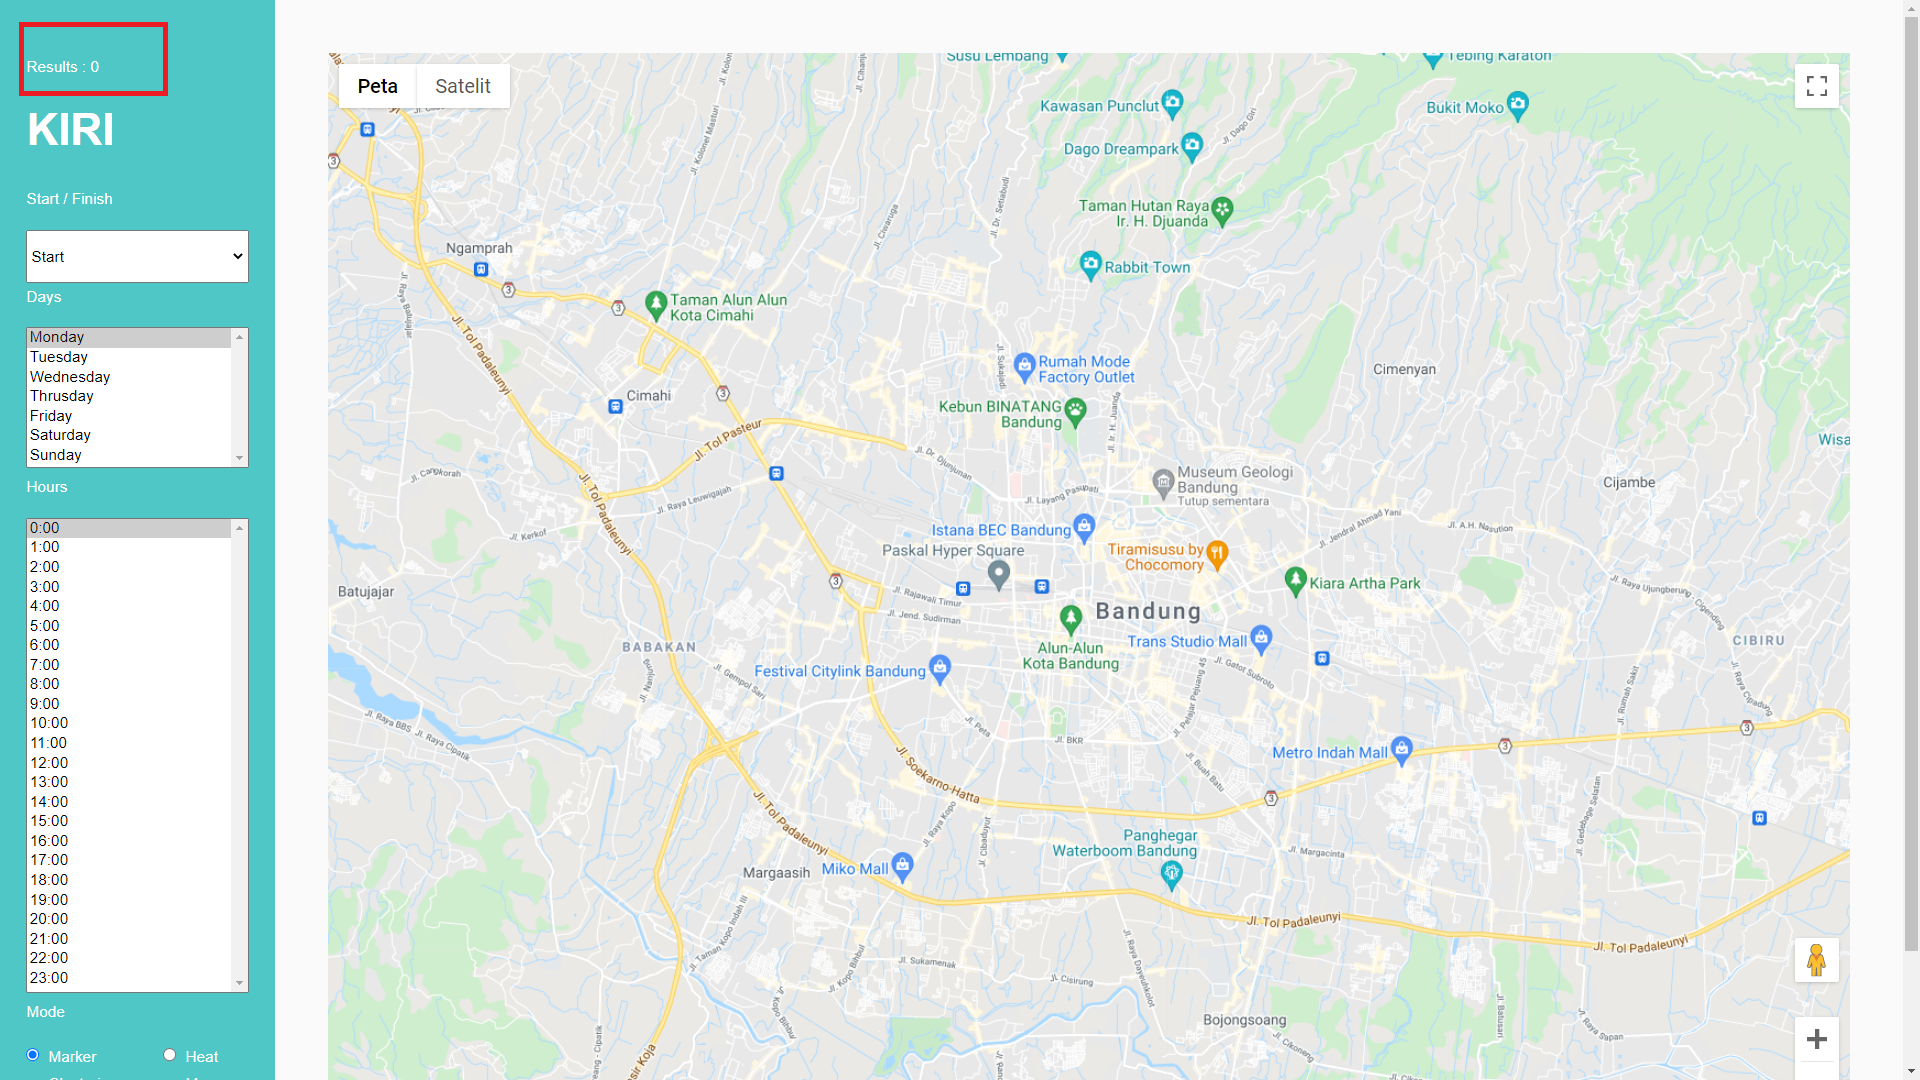
\includegraphics[scale=0.3]{Gambar/pengujian/result_helper.png}  
	\caption[parameter tambahan]{Parameter Tambahan} 
	\label{fig:testingState}
	\end{figure}
	

\subsubsection{Pengujian 1: Bagaimana penggunaan perangkat lunak KIRI pada saat jam kerja?}
\label{subsec:pengujian1}
Pada datalog yang tersedia dapat diketahui bahwa hasil log tersebut diambil pada tahun 2014. Kita dapat mengasumsikan bahwa jadwal kerja yang berlaku pada saat itu adalah dari pukul 06:00 - 18:00. Berdasarkan informasi tersebut kita akan melakukan observasi pada hari senin sampai jumat dari jam 06:00 - 18:00. Hasil dari pengjuan dapat dilihat pada gambar \ref{fig:operasional}.
  \begin{figure}[H]
	\centering  
	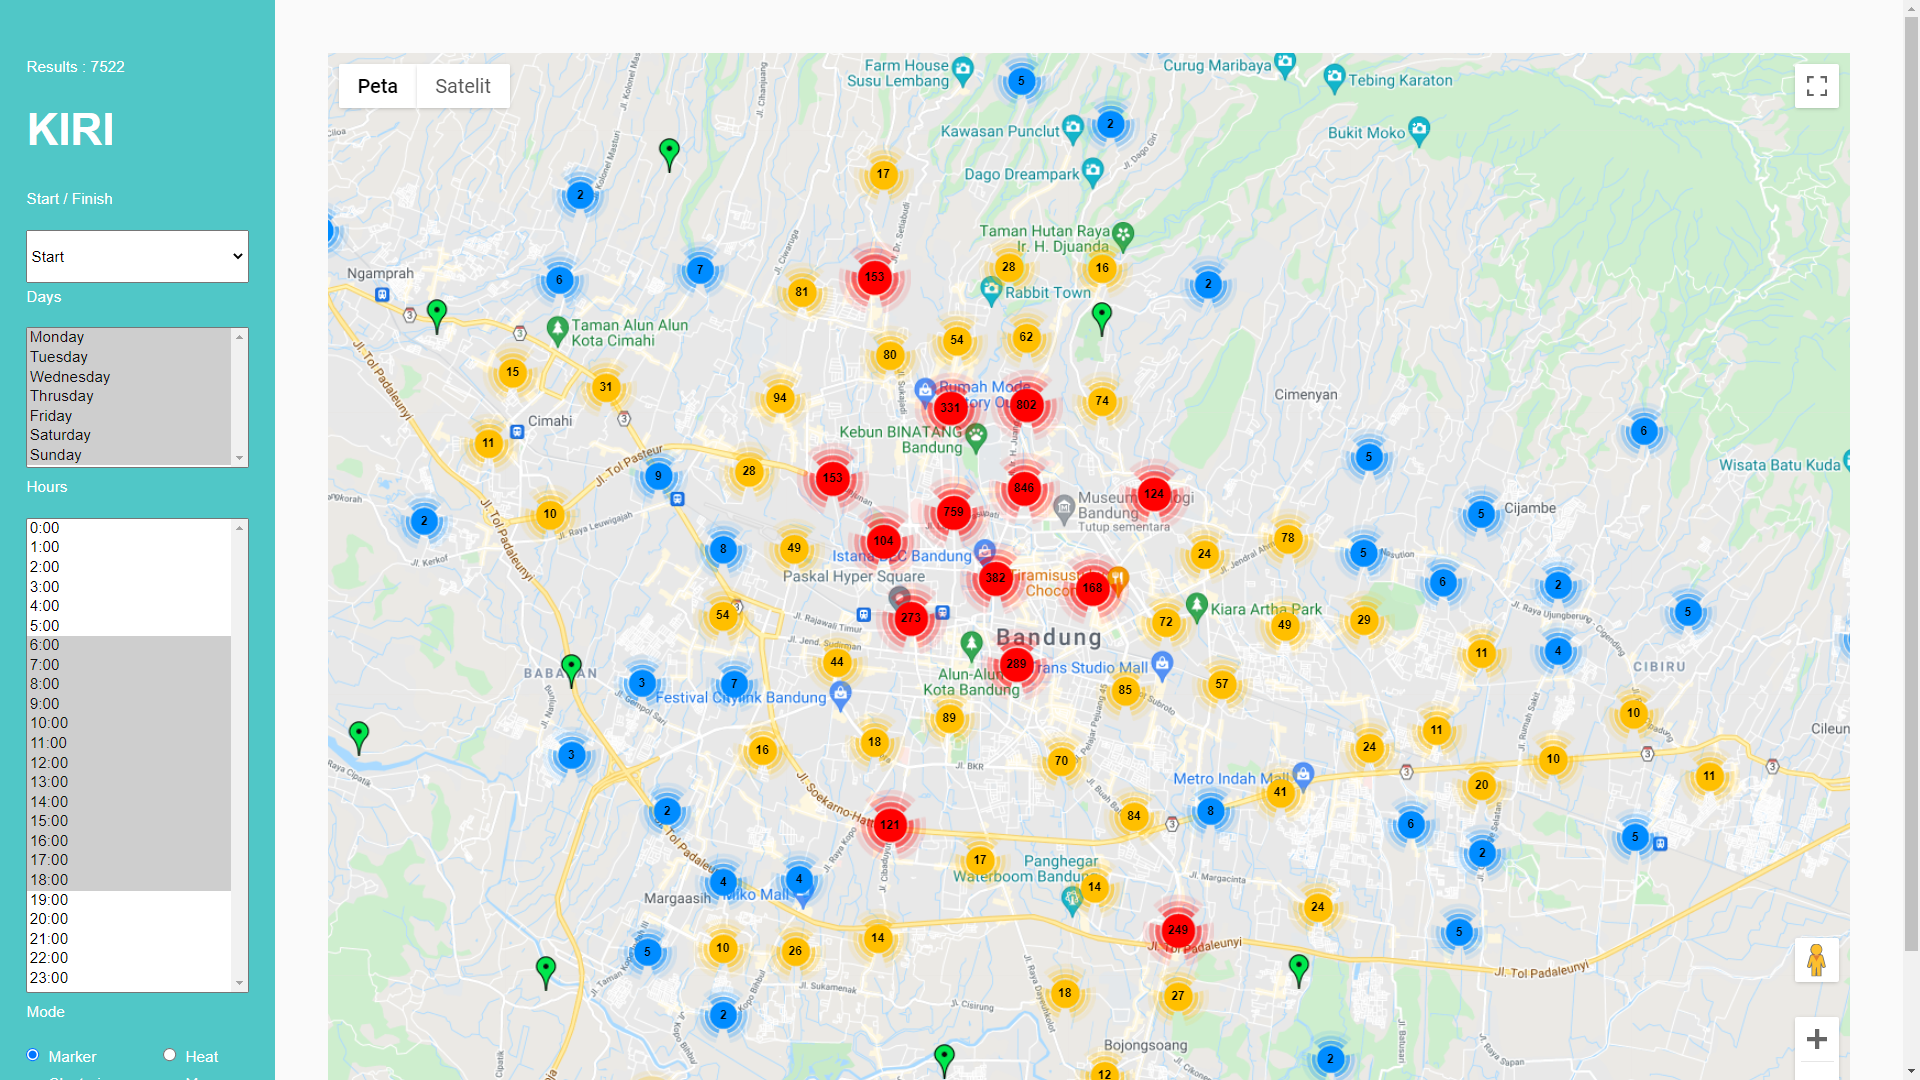
\includegraphics[scale=0.3]{Gambar/pengujian/senin-sabtu-operasional.png}  
	\caption[Senin-Sabtu Operasional]{Senin-Sabtu Jam Kerja} 
	\label{fig:operasional}
\end{figure}

Berdasarkan hasil observasi pada gambar \ref{fig:operasional} terdapat pemanggilan data sebanyak 7522 kali.


\subsubsection{Pengujian 2: Bagaimana penggunaan perangkat lunak KIRI pada saat non-jam kerja?}
\label{subsec:pengujian2}
Pada datalog yang tersedia akan dilakukan observasi untuk melihat jumlah penggunaan perangkat lunak KIRI pada jam non-operasional angkutan umum. Jam non-kerja dapat kita asumsikan dari pukul  19:00-07:00.
\begin{figure}[H]
	\centering  
	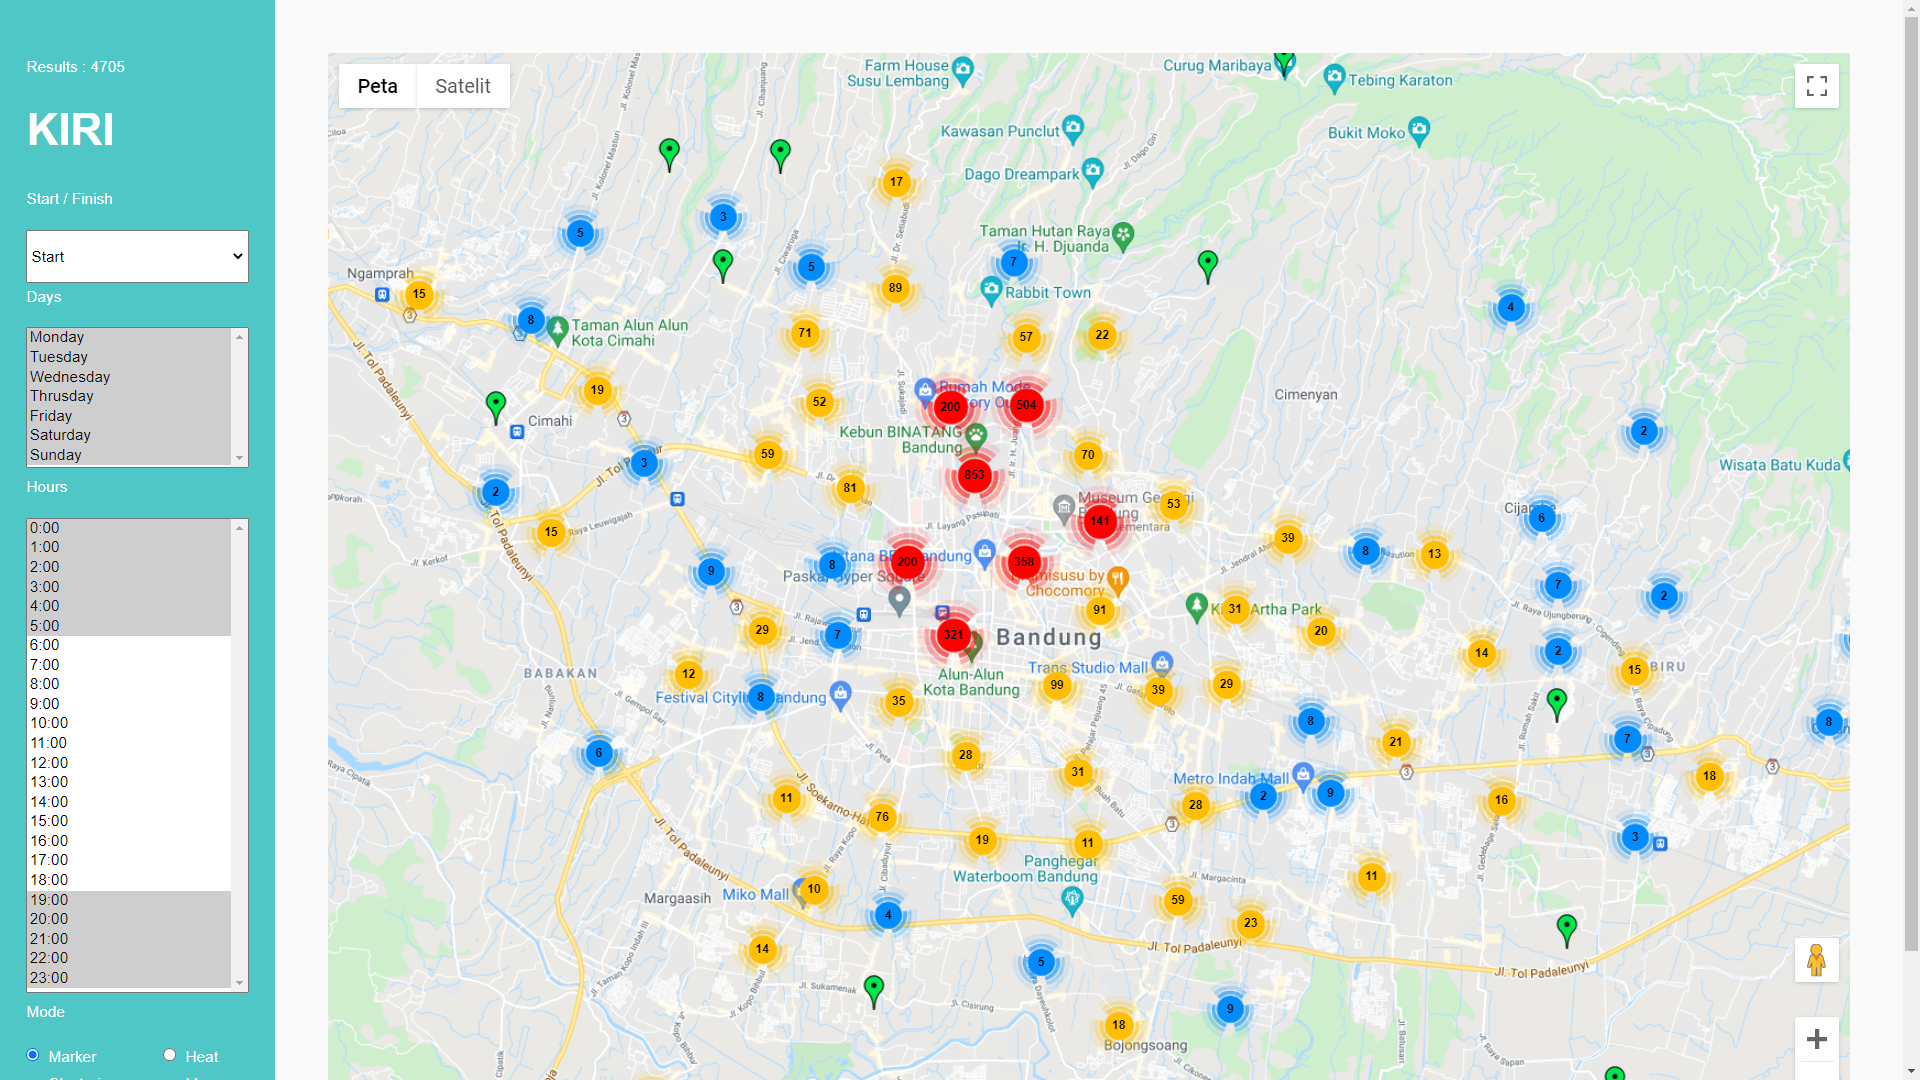
\includegraphics[scale=0.3]{Gambar/pengujian/senin-sabtu-non-operasional.png}  
	\caption[Senin-Sabtu Non Operasional]{Senin-Sabtu Non Jam Kerja} 
	\label{fig:nonOperasional}
\end{figure}

Berdasarkan hasil observasi pada gambar \ref{fig:nonOperasional} terdapat pemanggilan data sebanyak 4705 kali.

\subsubsection{Pengujian 3: Daerah manakah paling sering dijadikan titik awal pencarian rute?}
\label{subsec:pengujian3}
\begin{figure}[H]
	\centering  
	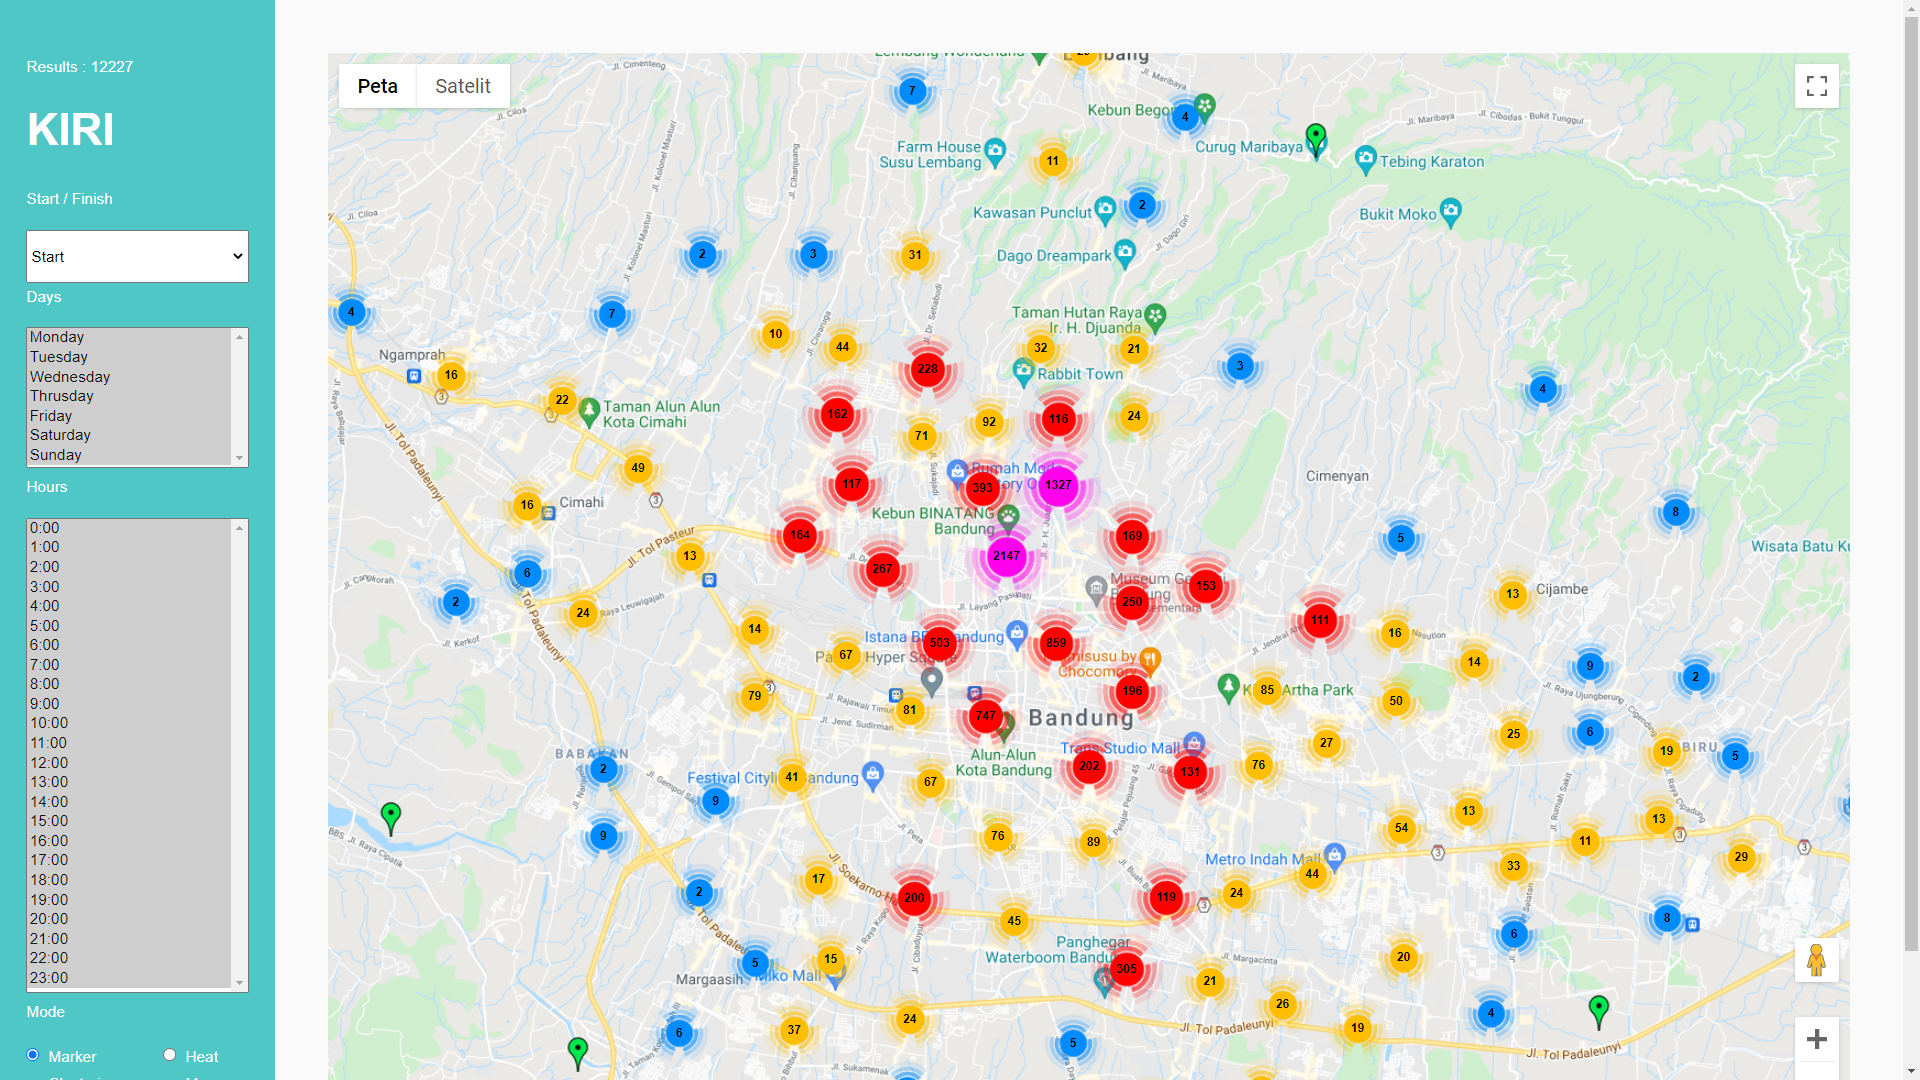
\includegraphics[scale=0.3]{Gambar/pengujian/titik-tujuan-terbanyak.png}  
	\caption[Daerah titik awal terbanyak]{Daerah titik awal terbanyak } 
	\label{fig:titkAwal}
\end{figure}
Berdasarkan gambar \ref{fig:titkAwal} dapat dilihat terdapat satu daerah yang memiliki jumlah pencarian terbanyak sebanyak 2147 kali. Ketika dilakukan observasi lebih lanjut dapat diketahui bahwa daerah tersebut adalah daerah Taman Sari seperti pada Gambar \ref{fig:tamanSari}.

\begin{figure}[H]
	\centering  
	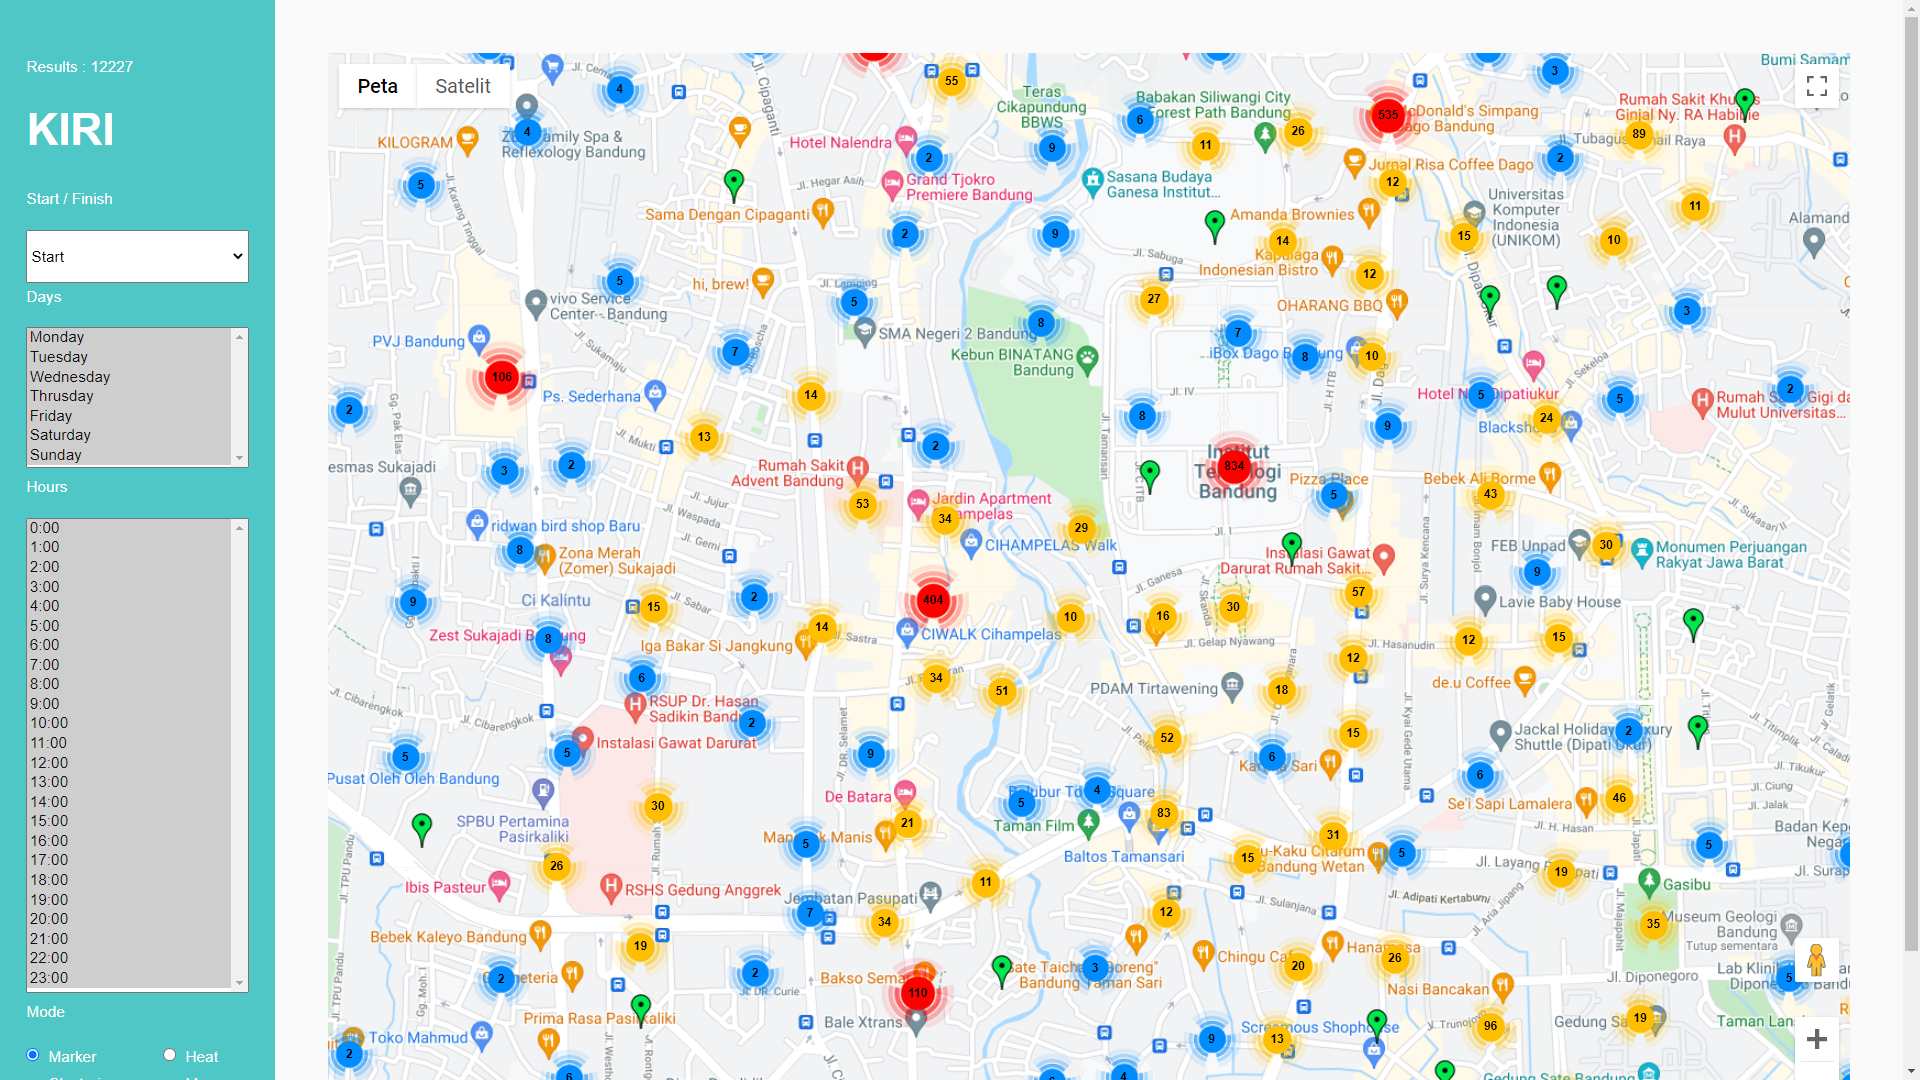
\includegraphics[scale=0.3]{Gambar/pengujian/taman-sari.png}  
	\caption[Daerah Taman Sari]{Daerah Taman Sari} 
	\label{fig:tamanSari}
\end{figure}

Berdasarkan hasil visualisasi pada gambar \ref{fig:tamanSari} akan dilakukan proses observasi lebih dalam untuk daerah Taman Sari yang dapat dilihat pada gambar \ref{fig:tamanSariZoom}.
\begin{figure}[H]
	\centering  
	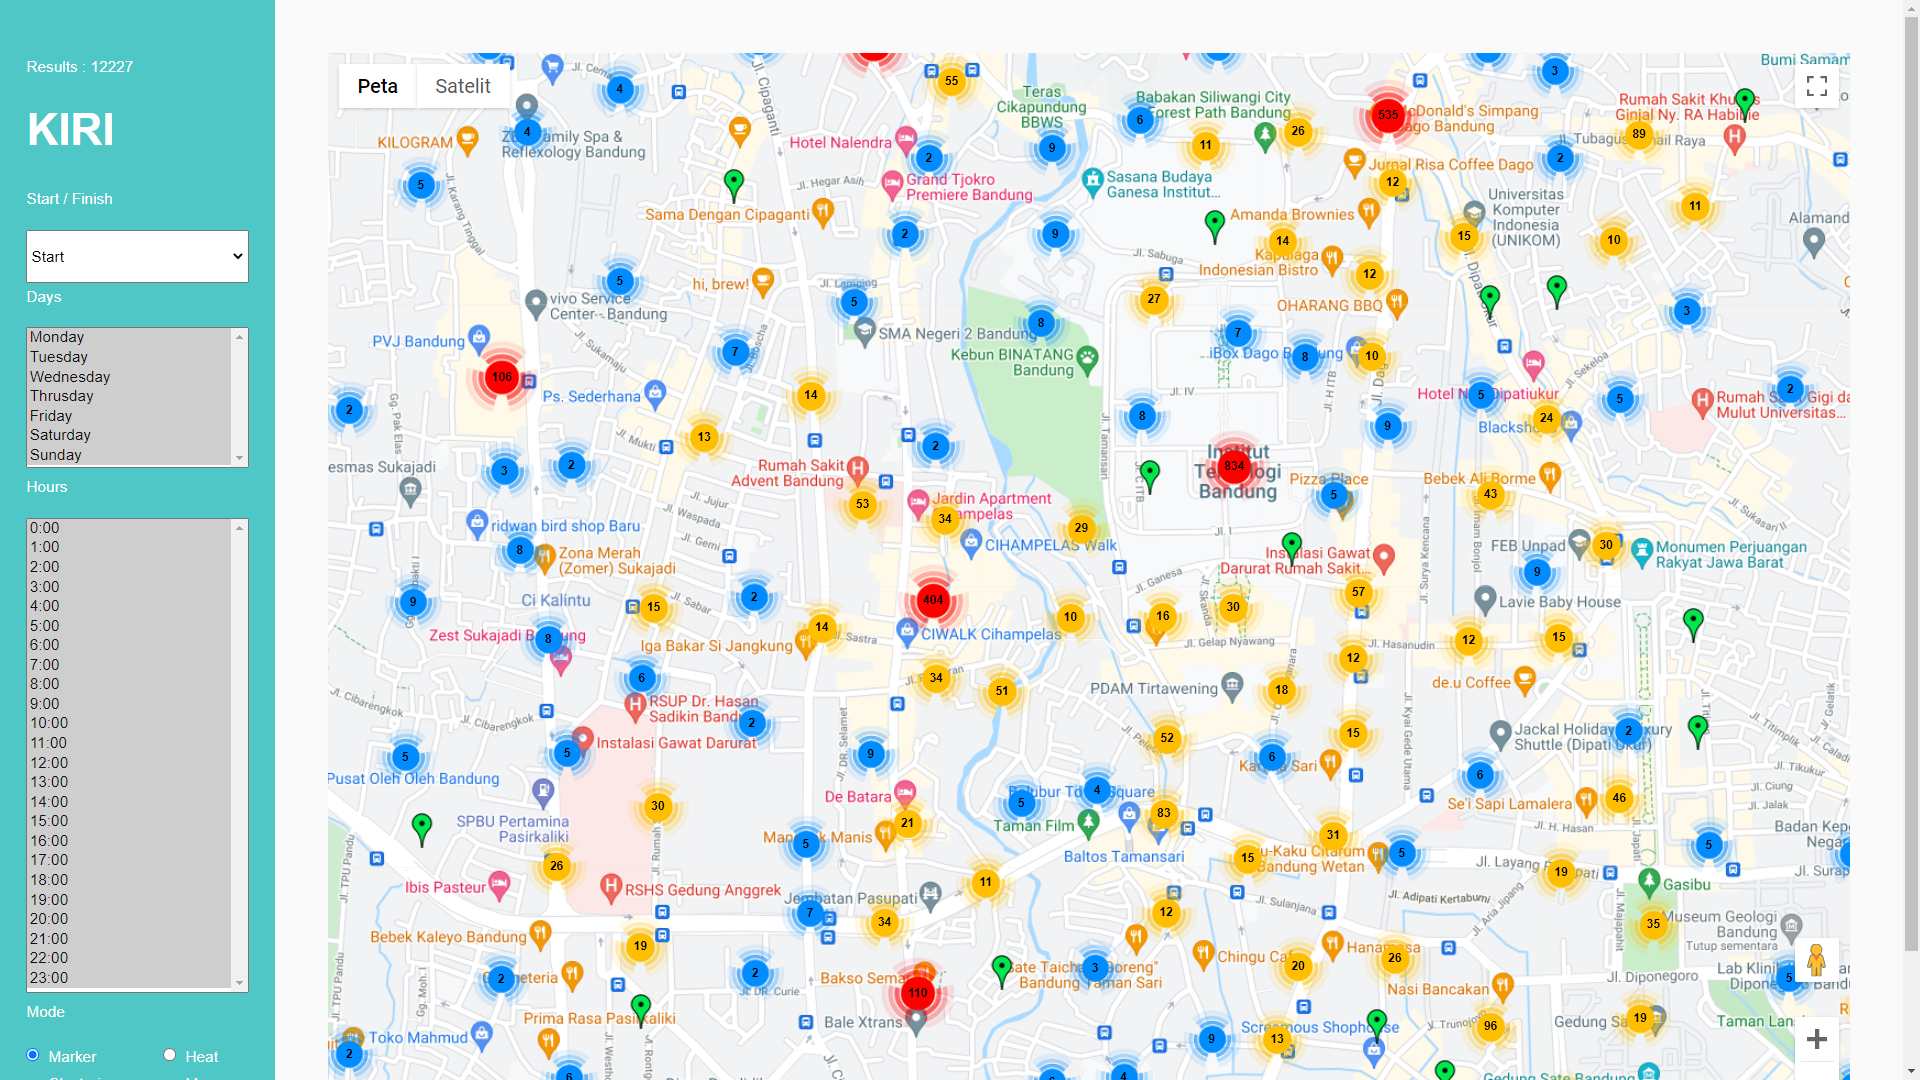
\includegraphics[scale=0.3]{Gambar/pengujian/taman-sari.png}  
	\caption[Daerah Taman Sari Zoomed]{Daerah Taman Sari Zoomed} 
	\label{fig:tamanSariZoom}
\end{figure}

Berdasarkan gambar \ref{fig:tamanSariZoom} terdapat lima daerah yang paling sering dijadikan titik awal pencarian rute. Daerah tersebut adalah   Paris Van Java , Cihampelas Walk, Institut Teknologi Bandung (ITB), dan McDonald's Simpang Dago. Untuk memperkecil hasil pencarian mode visualisasi akan diganti menjadi \textit{heat map}. Hal ini dilakukan agar dapat melihat titik-titik yang intensitas terbesar. 

\begin{figure}[H]
	\centering  
	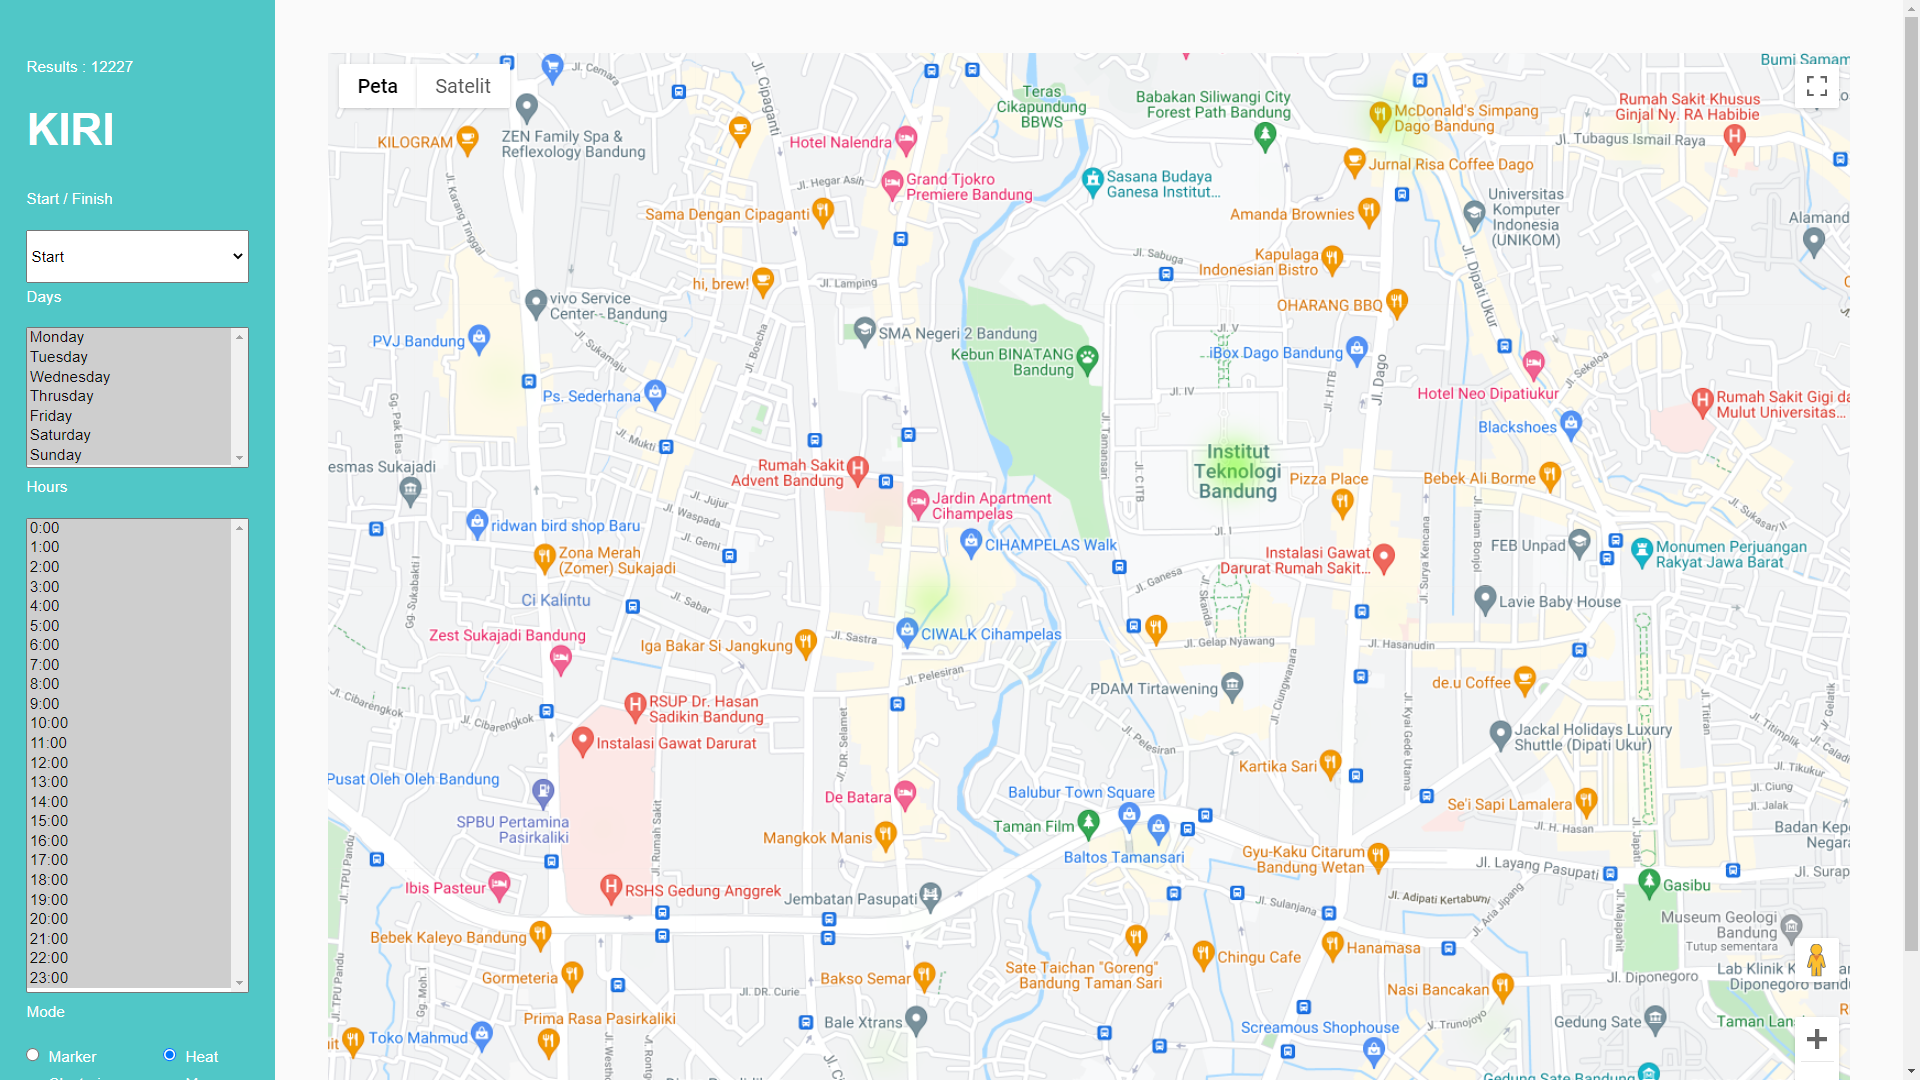
\includegraphics[scale=0.3]{Gambar/pengujian/hasil-heat-map.png}  
	\caption[Heat Map Taman Sari]{Heat Map Taman Sari} 
	\label{fig:heatMapTamanSari}
\end{figure}

Berdasarkan gambar \ref{fig:heatMapTamanSari} dapat disimpulkan bahwa titik yang menjadi tempat tujuan terbanyak adalah Institut Teknologi Bandung (ITB).

\subsubsection{Pengujian 4: Daerah manakah paling sering dijadikan tujuan akhir pencarian rute?}
\label{subsec:pengujian4}
\begin{figure}[H]
	\centering  
	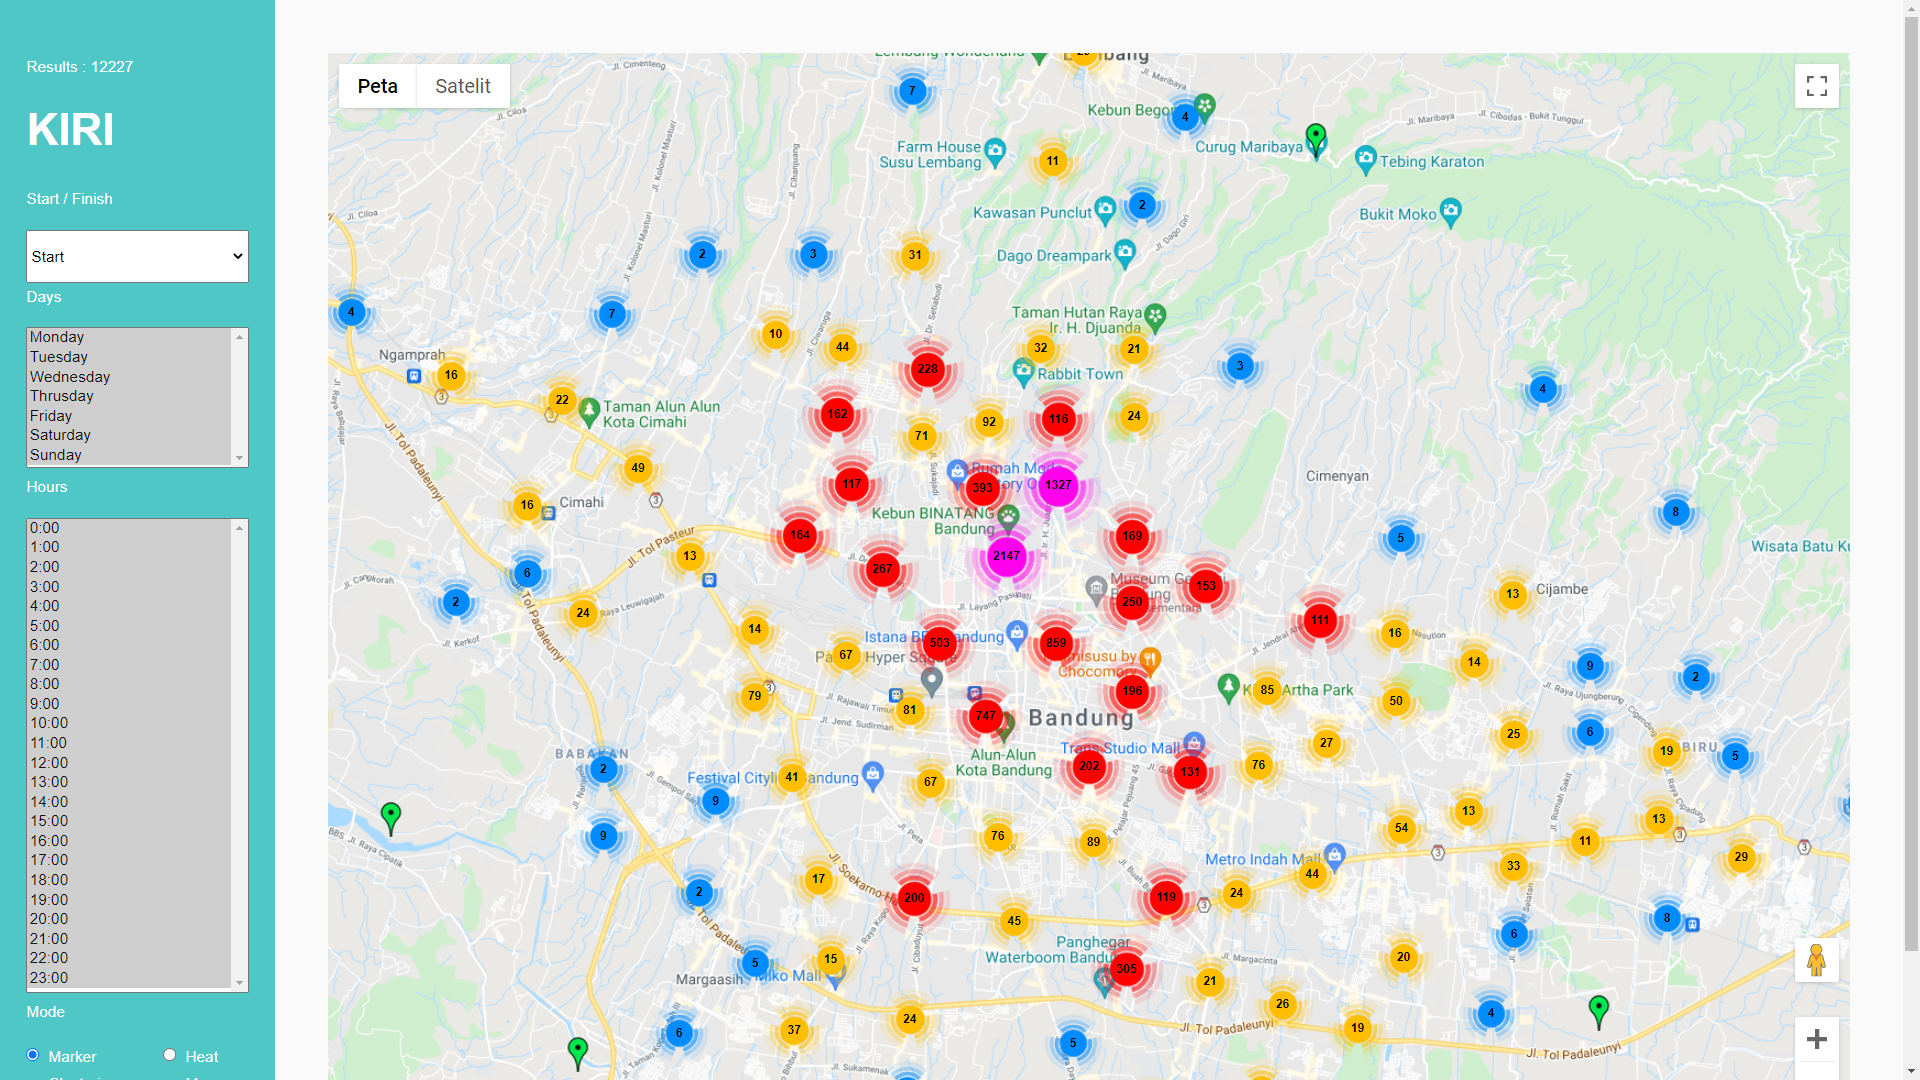
\includegraphics[scale=0.3]{Gambar/pengujian/titik-tujuan-terbanyak.png}  
	\caption[Daerah titik tujuan terbanyak]{Daerah titik tujuan terbanyak} 
	\label{fig:titikTujuan}
\end{figure}

Berdasarkan gambar \ref{fig:titikTujuan} dapat dilihat terdapat satu daerah yang memiliki jumlah pencarian terbanyak sebanyak 1350 kali. Ketika dilakukan observasi lebih lanjut dapat diketahui bahwa daerah tersebut adalah daerah Braga City Walk. Untuk mendapatkan hasil yang lebih mendetail akan dilakukan proses observasi lebih dalam untuk daerah Braga City Walk yang dapat dilihat pada gambar \ref{fig:bragaZoom}.

\begin{figure}[H]
	\centering  
	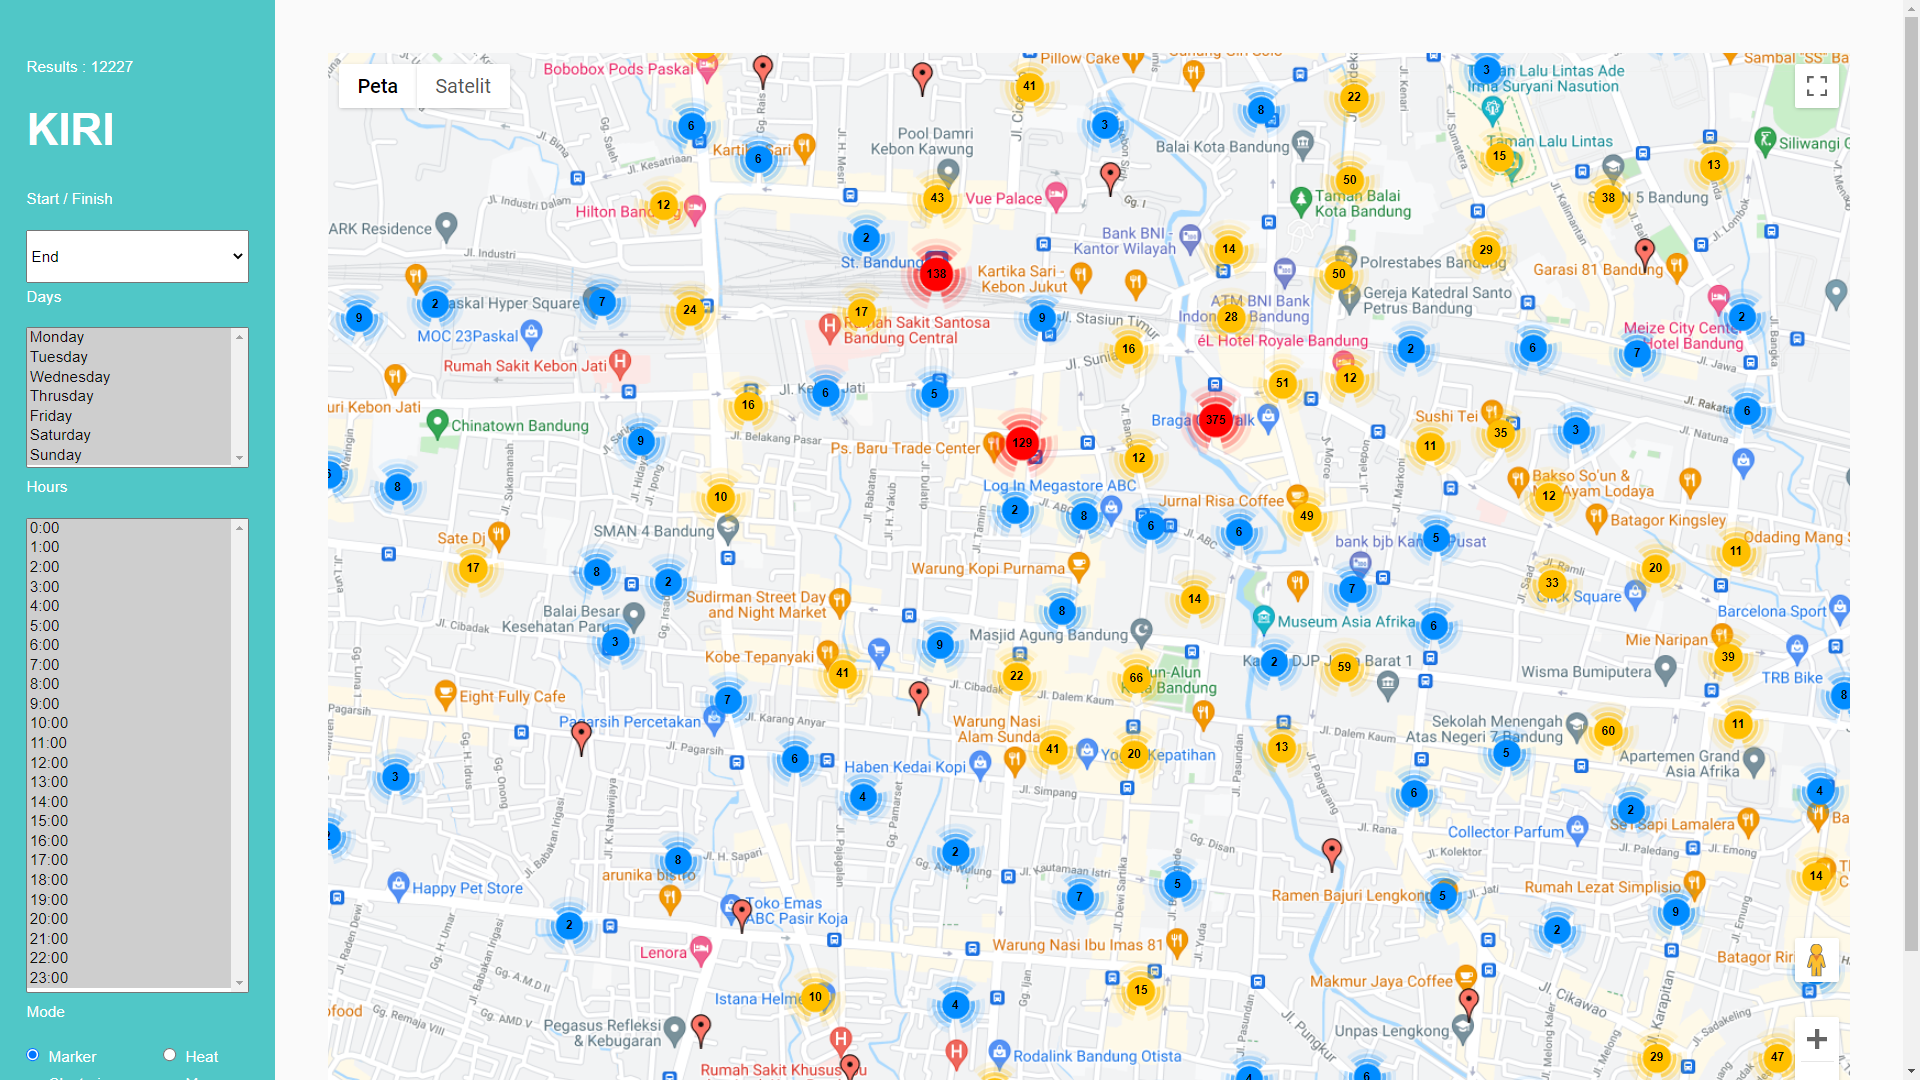
\includegraphics[scale=0.3]{Gambar/pengujian/bragaZoom.png}  
	\caption[Gambar Daerah Braga ]{Gambar Daerah Braga } 
	\label{fig:bragaZoom}
\end{figure}

Berdasarkan hasil gambar \ref{fig:bragaZoom} terdapat tiga titik yang paling sering menjadi destinasi tujuan pengguna perangkat lunak KIRI. titik tersebut ialah Stasiun Bandung, Braga City Walk, dan Pasar Baru Trade Center.

\subsubsection{Pengujian 5: Daerah manakah paling sering dijadikan titik awal pencarian rute pada saat \textit{weekend}?}
\label{subsec:pengujian5}
\begin{figure}[H]
	\centering  
	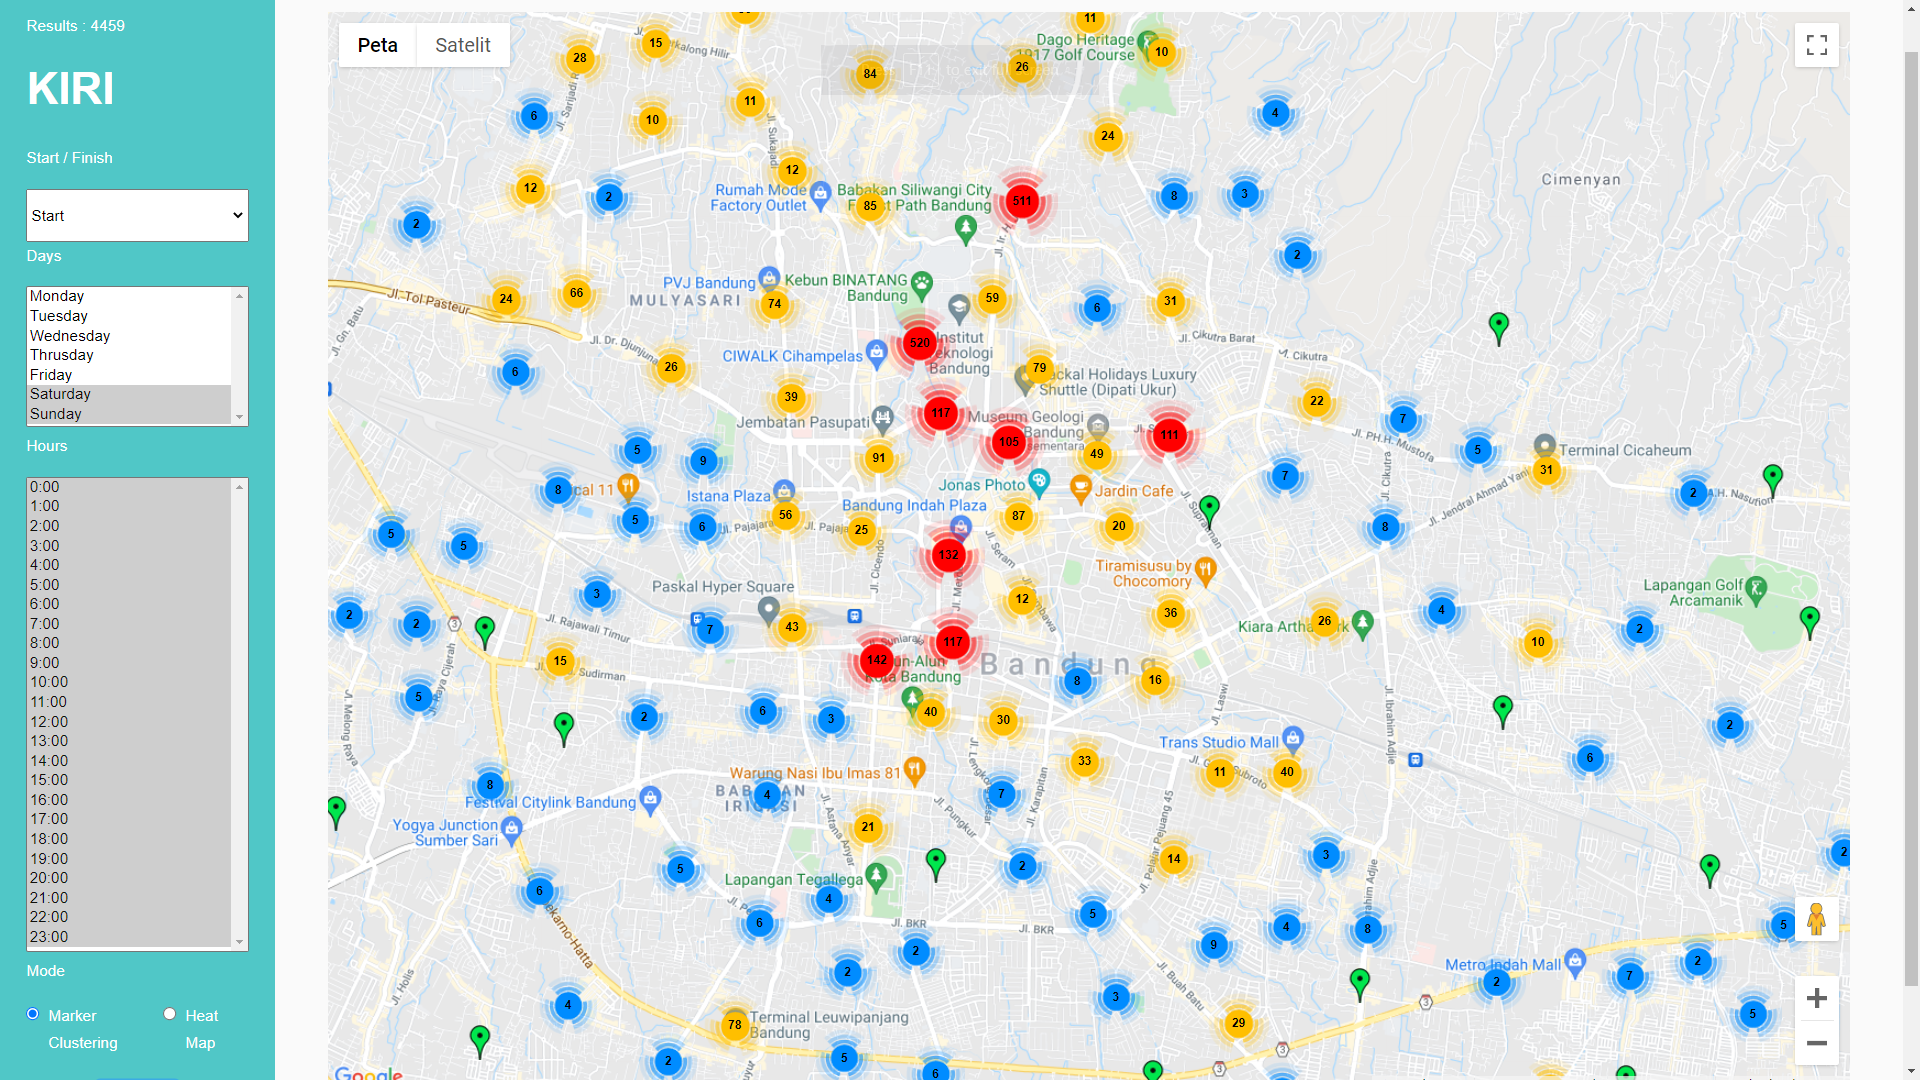
\includegraphics[scale=0.3]{Gambar/pengujian/weekend-start.png}  
	\caption[Daerah dengan titik start pada saat weekend]{Daerah dengan titik start pada saat weekend } 
	\label{fig:weekendStart}
\end{figure}

Berdasarkan gambar \ref{fig:weekendStart} dapat dilihat terdapat satu daerah yang memiliki jumlah pencarian terbanyak sebanyak 775 kali. Ketika dilakukan observasi lebih lanjut dapat diketahui bahwa daerah tersebut merupakan daerah Taman Sari.

\begin{figure}[H]
	\centering  
	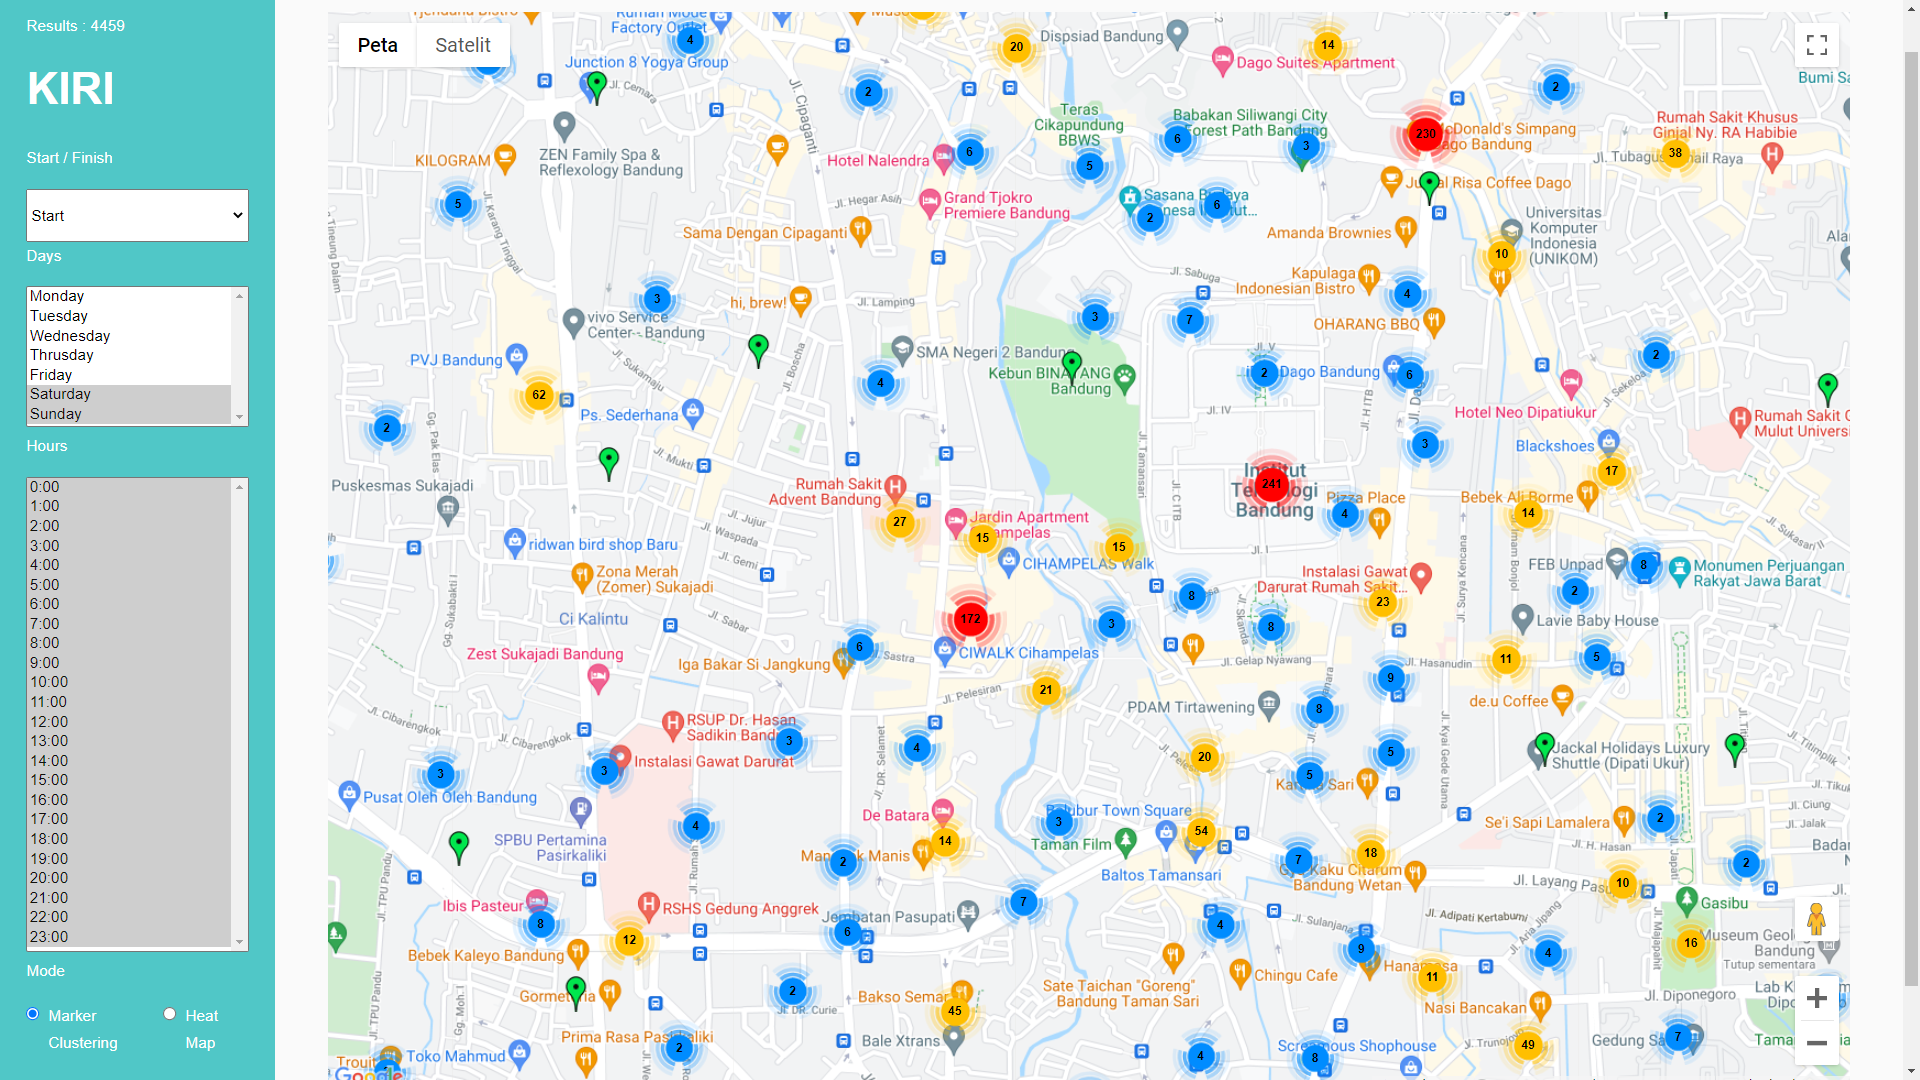
\includegraphics[scale=0.3]{Gambar/pengujian/weekend-taman-sari-zoomed.png}  
	\caption[Daerah Taman Sari Weekend ]{Daerah Taman Sari Weekend } 
	\label{fig:weekendStartZoom}
\end{figure}

Ketika dilakukan observasi lanjutan seperti pada gambar \ref{fig:weekendStartZoom}, dapat terdapat tiga hotspot yang paling sering dijadikan tempat awal rute pencarian tempat ini adalah Cihampelas Walk, Institut Teknologi Bandung (ITB), dan McDonald's Simpang Dago.


\subsubsection{Pengujian 6: Daerah manakah paling sering dijadikan titik tujuan pencarian rute pada saat \textit{weekend}?}
\label{subsec:pengujian6}

\begin{figure}[H]
	\centering  
	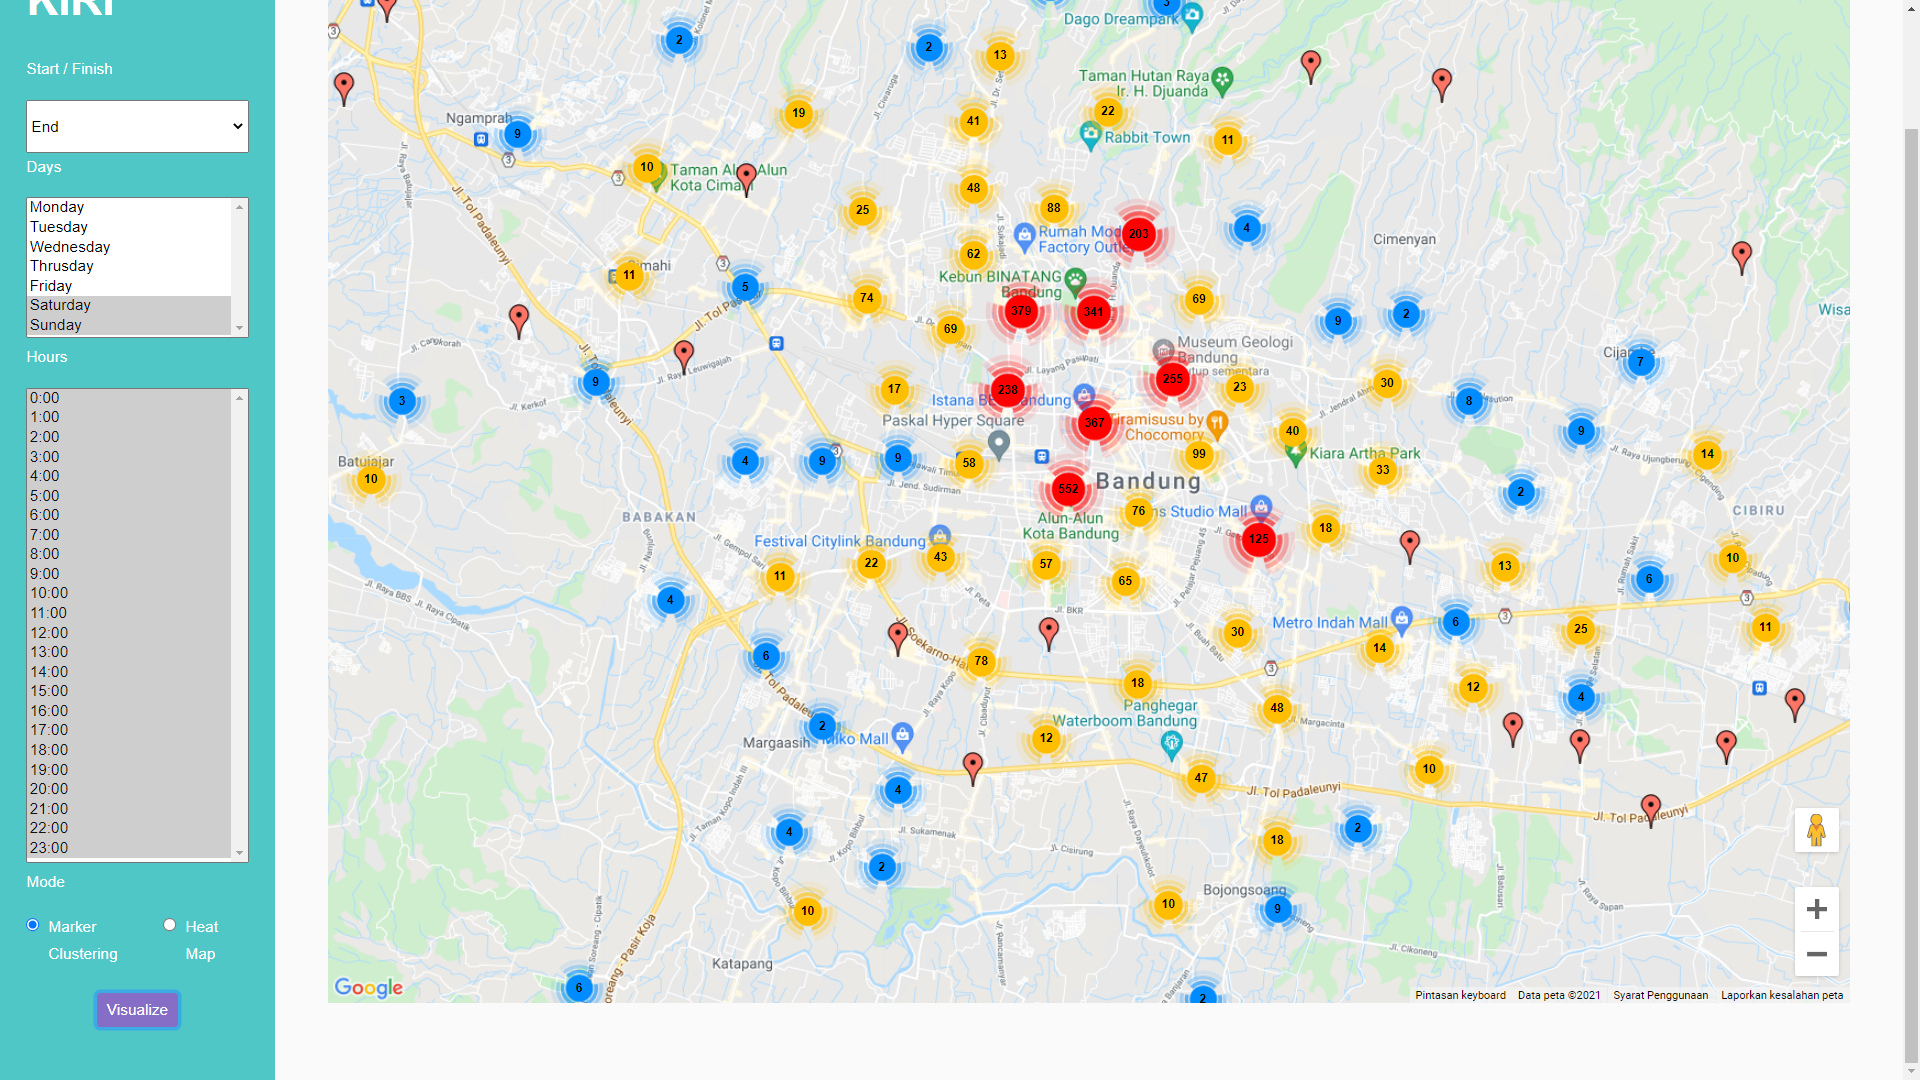
\includegraphics[scale=0.3]{Gambar/pengujian/weekend-end.png}  
	\caption[Daerah dengan titik tujuan pada saat weekend]{Daerah dengan titik tujuan pada saat weekend } 
	\label{fig:weekendEnd}
\end{figure}
Berdasarkan gambar \ref{fig:weekendEnd} dapat dilihat terdapat satu daerah yang memiliki jumlah pencarian terbanyak sebanyak 551 kali. Ketika dilakukan observasi lebih lanjut dapat diketahui bahwa daerah tersebut merupakan daerah Alun-Alun Kota Bandung.

\begin{figure}[H]
	\centering  
	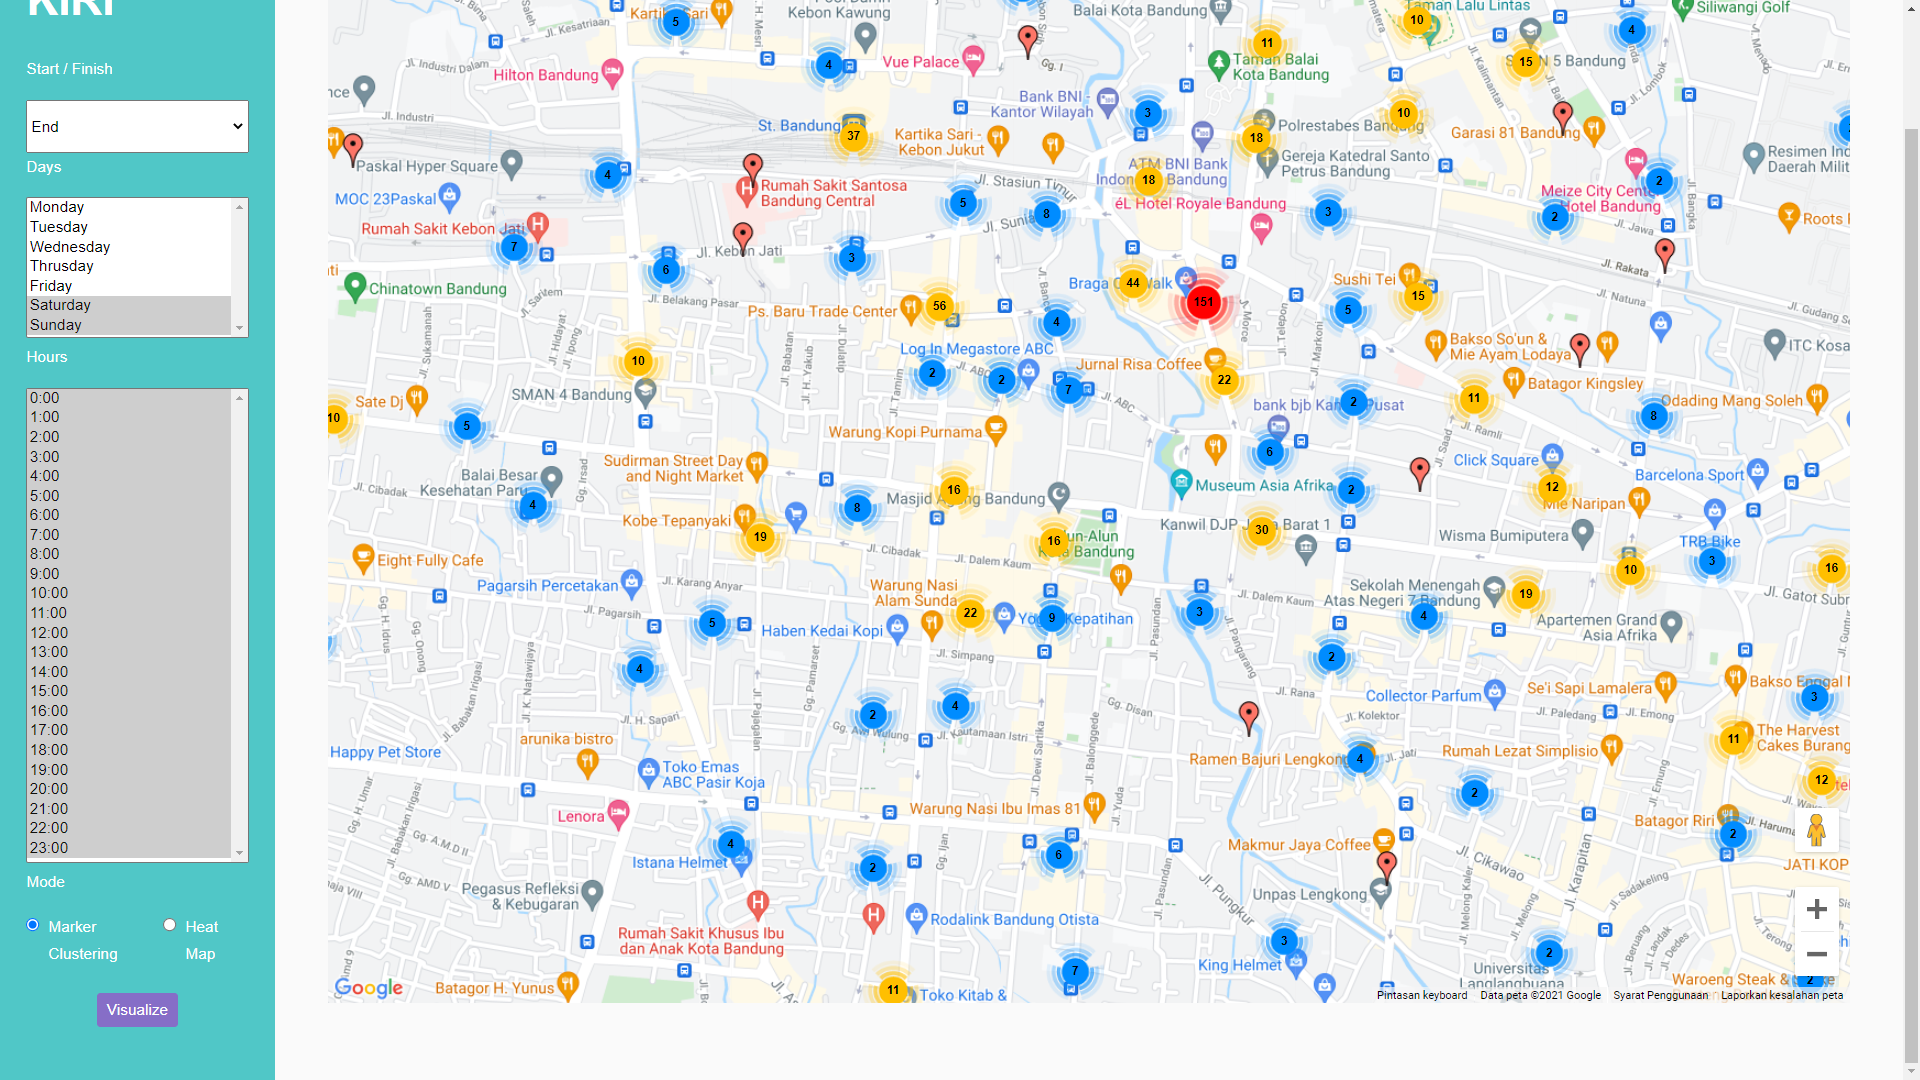
\includegraphics[scale=0.3]{Gambar/pengujian/weekend-end-zoomed.png}  
	\caption[Daerah Alun Alun Kota Bandung ]{Daerah Alun Alun Kota Bandung } 
	\label{fig:weekendEndZoomed}
\end{figure}

Ketika dilakukan observasi lanjutan seperti pada gambar \ref{fig:weekendEndZoomed}, dapat terdapat sebuah hotspot yang paling sering dijadikan tempat tujuan akhir rute pencarian tempat ini adalah Cafe Jurnal Risa.




\section{Masalah yang Dihadapi saat Implementasi}
Penulis memiliki beberapa masalah yang dihadapi dalam   pengembangan aplikasi visualisasi data histori KIRI menggunakan \textit{Google Maps Javascript API}:
\begin{enumerate}
	\item Perlu dilakukan proses pembatasan data, hal ini dikarenakan data histori yang diberikan sangatlah luas bahkan mencakup pencarian rute untuk daerah Jakarta. Hal ini mengakibatkan mode visualisasi \textit{heat map} kurang dapat memberikan informasi dikarenakan persebaran data yang terlalu banyak.
	
	\item Pengujian pada perangkat lunak ini hanya berdasarkan tiga atribut yaitu tempat awal / tempat tujuan, hari, dan jam, dan belum mencakup atribut seperti tanggal, bulan, tahun.
	
	\item Dataset yang diberikan meruapakan \textit{data log} yang tercatat pada tahun 2014 sehingga ada beberapa hotspot yang mungkin saja sudah tidak relevan dengan keadaan saat ini.
	
	\item Proses \textit{functional testing} tidak dapat dilakukan secara maksimal dikarenakan adanya limitasi penggunaan API dari pihak \textit{Google}.
	
	
\end{enumerate}